\chapter[Page Eviction Strategies]{Page Eviction Strategies in the Context of Pointer Swizzling} \label{ch:eviction}

\section{Importance of Page Eviction Strategies} \label{sec:evictionreasons}

    As discussed in subsection \ref{subsec:reasonhitrate}, it's the main goal of the buffer pool to \emph{maximise the hit rate} as a high hit rate drastically increases the performance of the whole DBMS. 

    It was already discussed that the used page replacement strategy needs to be optimized to achieve this goal. The optimal OPT algorithm is only of use in theory as it cannot be implemented but it defines the desired characteristics of actually realizable page replacement algorithms. They should evict the page that won't be used for the longest time in the near future. But as they only know about the page references of the past, they only approximate this behavior by \emph{assigning reuse probabilities} to the pages in the buffer pool \emph{based on statistics} about the page accesses.

    One very common page replacement algorithm is the \emph{LRU} (least recently used) strategy which expects a page that wasn't used for the longest time in the past to be used (more details about the definition of usage in the next section) the furthest in the future. But many page reference strings (sequence of page reference) doesn't perform well with this page replacement algorithm. A loop that accesses exactly the number of pages that fit in the buffer pool will work perfectly as already after the first iteration there are only pages in the buffer pool that were referenced during the loop (if there aren't concurrent transactions using other pages) as the pages referenced before the loop are always accessed earlier than the ones accesses during the loop. As any further page references that happen during the loop only access pages that already reside in the buffer pool, there will only be page hits for the rest of the time the loop is running. But if there is one more page referenced during the loop, the hit rate will drop to $0$. When the last page of the loop will be referenced, the buffer pool will already only contain pages accessed during the loop and therefore the first page referenced during the loop will be evicted to free a frame for the last page of the loop. The next page reference will cause the just evicted page to be retrieved from the secondary storage again and it will replace the second page referenced during the loop. And therefore every page reference during the loop will be a page miss. A more sophisticated page replacement algorithm would recognize the loop and it could reduce the physical page references to \num{2} during each iteration of the loop after the first iteration. But the reason why page replacement algorithms which only rely on recency are still popular can be seen in figure \ref{fig:lrulocality}. It shows a situation in which a buffer pool with \num{1095} buffer frames could achieve a hit rate of \SI{75}{\percent} using LRU page replacement. The used database had a size of \num{1691576} pages and only the locality of the page references allowed the buffer pool to achieve such a high hit rate while storing only a small portion of the whole database. The presented situation is based on the reference string of the synthetic OLTP benchmark TPC-C. The LRU page replacement algorithm is usually implemented using a stack where a page is moved to the bottom of the stack when it is referenced and where the page at the top of the stack is evicted as this page wasn't moved down for the longest time. But there exist many modifications for this page replacement strategy focusing on either reducing the weaknesses of this strategy with regard to miss rates of some specific reference strings (e.g. LRU-k proposed in \cite{ONeil:1993}) or reducing the complexity (due to synchronization) of the operations performed to update the statistics during a page hit (e.g. CLOCK).

\begin{@empty}
    \tikzset{%
        every node/.style = {font = \sffamily},
        phantom/.style = {rectangle, draw = none, thick},
        layer/.style = {rectangle, draw, thick},
        toplayers/.style = {layer},
        buffer/.style = {layer},
        storage/.style = {layer},		
        disk/.style = {cylinder, cylinder uses custom fill, shape border rotate = 90, draw, minimum height = 1cm, minimum width = 1.5cm, thick},
        disktext/.style = {},
        interfacearrow/.style = {<->, thick, draw = black}
    }

    \begin{figure}[ht!]
        \centering
        \resizebox{\textwidth}{!}{
            \begin{tikzpicture}
                \begin{axis}[title = {TPC-C with Warehouses: 100, Threads: 25},
                           axis on top,
                 		   width = \textwidth,
                           height = .25\textheight,
                           xlabel = {LRU stack depth},
                           xlabel near ticks,
                           xmode = log,
                           xmin = 5e-1,
                           xmax = 1e8,
                           ymode = normal,
                           ybar interval,
                           x tick label as interval = false,
                           xtick = {},
                           xtickten = {0, 1, ..., 8},
                           scaled y ticks = false,
                           ylabel = {\# of references},
                           ylabel near ticks,
                           grid = none]
                    \addplot [fill = gray!50] table [x = Lower, y = Count] {./tex/data/lru_stackdepth_histograms/tpcc/ln_histogram_lrused_stackdepth/ln_histogram_LRUsed_stackdepth_analysis_wh100_t25.csv};
                \end{axis}
            \end{tikzpicture}
        }
        \caption{The LRU (least recently used) stack depth distribution for 25 parallel transactions (threads). The basis of this data is a reference strings with the length of \num{66161654} generated by executing the TPC-C benchmark with a database of 100 warehouses. The benchmark simulates 25 users concurrently querying the database. The LRU stack depth of a page reference is the number of different page references between this page reference and the most recent fix of the same page. If a page is fixed twice without another page fix in between, the second of those page references will have a LRU stack depth of $1$. Each of the page references is assigned to one of the histogram buckets by its LRU stack depth and therefore the height of the leftmost bar of the histogram indicates the number of page references with a LRU stack depth of 1.}
        \label{fig:lrulocality}
    \end{figure}
\end{@empty}

    Another proposed page replacement strategy uses the total number of references to a specific page to pick a victim for eviction. The \emph{LFU} (least frequently used) algorithm maintains a counter for each frame of the buffer pool counting the number of references of the contained page. The counter is initialized with \num{1} when the frame gets allocated to a page and it will be increased with every further reference of that page as long as the page stays in the buffer pool. This page replacement expects the most frequently used pages to be used the most in the recent future. But this strategy is even easier to break than the LRU page replacement strategy. A page that was referenced very frequently for some time but without any references in the recent past (might be a long time) stays in the buffer pool as long as there aren't enough pages with a higher number of references. Therefore there can be a large number of pages in the buffer pool that just waste buffer frames as they won't be used anymore in the future but as the further page reference string doesn't contain pages that are accessed that frequently, they cannot be evicted. This problem prevents this page replacement algorithm from being used but many other page replacement algorithms combine the idea of taking into account the frequency of references with the usage of other statistical data (e.g. LRD-V1 (least reference density) as proposed in \cite{Effelsberg:1984}).

        Techniques that aren't usually recognized as being part of the page replacement algorithms are \emph{memory allocation strategies} (as discussed in subsection \ref{subsec:allocation}) which is implicitly done by the page eviction and \emph{prefetching strategies} which also decide about the pages that are actually cached in the buffer pool. The usual way of selecting pages to be cached in the buffer pool is called \emph{demand fetching} as a page is cached on demand (on a page reference). Prefetching tries to estimate pages that weren't used in the recent past but that will be referenced next by recognizing patterns in the recorded page reference string or by receiving hints from the upper layers of the DBMS.

    The introduction of two basic page replacement strategies LRU and LFU shows the vitally of selecting a page replacement strategy that matches best the expected workload. Page replacement algorithms in general can be classified with regard to the used statistics about the reference history of a page like it was done in \cite{Effelsberg:1984} as shown in figure \ref{tab:pagereplaceclassification}. More recent and quite promising page replacement algorithms are presented and evaluated in this chapter and an overview of many others can be found in \cite{Datenbanksysteme_-_Konzepte_und_Techniken_der_Implementierung}, \cite{Datenbanken_-_Implementierungstechniken}, \cite{Wenguang:2001} or \cite{Paajanen:2007}.

\begin{@empty}
    \begin{table}[h]
        \centering
        \small
        \begin{tabular}{|c|c|c|c|c|}
            \hline
            \multicolumn{2}{|c|}{\multirow{2}{*}{\textbf{\begin{tabular}[c]{@{}c@{}}Consideration during\\ selection decision\end{tabular}}}}	&	\multicolumn{3}{c|}{\textbf{Age}}	\\ \cline{3-5} 
            \multicolumn{2}{|c|}{}	& \textbf{\begin{tabular}[c]{@{}c@{}}No \\ consideration\end{tabular}}	& \textbf{\begin{tabular}[c]{@{}c@{}}Since most \\ recent reference\end{tabular}}	& \textbf{\begin{tabular}[c]{@{}c@{}}Since first \\ reference\end{tabular}}	\\ \hline
            \multirow{4}{*}{\belowbaseline[2ex]{\rotatebox{90}{\textbf{References}}}}	& \textbf{\begin{tabular}[c]{@{}c@{}}No \\ consideration\end{tabular}}	& RANDOM	&	& FIFO	\\ \cline{2-5} 
                &	\textbf{\begin{tabular}[c]{@{}c@{}}Most recent\\ reference\end{tabular}}	&	&	\begin{tabular}[c]{@{}c@{}}LRU\\ CLOCK\\ GCLOCK-V2\end{tabular}	&	\\ \cline{2-5} 
                &	\multirow{2}{*}{\textbf{All references}}	&	\multirow{2}{*}{LFU}	&	\begin{tabular}[c]{@{}c@{}}GCLOCK-V1\\ DGCLOCK\end{tabular}	&	LRD-V1	\\
                &	&	&	\multicolumn{2}{c|}{\begin{tabular}[c]{@{}c@{}}LRU-K\\ LRD-V2\end{tabular}}	\\ \hline
        \end{tabular}
        \vspace{.5em}
        \caption[Classification of Classical Page Replacement Algorithms]{Classification of classical page replacement algorithms taken from \cite{Effelsberg:1984}.}
        \label{tab:pagereplaceclassification}
    \end{table}
\end{@empty}

\section[Problems of Page Eviction with Pointer Swizzling]{Problems of Page Eviction with Pointer Swizzling in the Buffer Management}

    Page replacement algorithms have the task of selecting a page, which resides in memory, to be evicted to free memory space for other pages to buffer in memory. In order to do so, this component of a buffer manager needs to know some features of the buffer pool. At least it needs to know about the address space of the buffer, to select a frame to be freed. In theory, those page replacement strategies \emph{select an arbitrary page} (following the specific algorithm) from the buffer pool for eviction without taking care about the usage of those pages. And even complex page replacement algorithms that store many statistics on each page in the buffer pool only update those statistics on a page fix (or on an unfix operation as well). 

\subsection[General Problems of the Implementation]{General Problems of the Implementation of Page Eviction Strategies}

    There are many limitations regarding the eviction of a page in a DBMS buffer manager. A page might be \emph{fixed for a very long time} (e.g. with an exclusive latch which prevents concurrent fixes) and therefore it might be already the least recently used page in a LRU strategy because the time of the last update of the LRU-stack was to long ago. The implementation of a page evictioner needs to take that into account and there needs to be some rules defined for such situations. In case of a LRU strategy, a page that is fixed might be considered as used and therefore it shouldn't be the least recently used page. But if a page is considered used during the whole time it is fixed, the replacement algorithm should continuously update the statistics about that page - at least in theory. Its trivial that this is impractical but the same result can be achieved by updating the statistics on an unfix as this is the last time it was used (proposed as least recently unfixed in \cite{Effelsberg:1984}). And before the unfix, the page couldn't be evicted and therefore the intention of the replacement strategy does hold here as well.

    The feature to \emph{pin a page} for a later refix, as it is implemented in Zero, is another of those problems. The \emph{pin for refix} is a performance optimization that allows a transaction to release the latch of a page without the need of fixing it again using the page ID as this would cause the fix operation to localize the page in the buffer pool using a hash table lookup (can be prevented using pointer swizzling as discussed in the previous chapters). It has the same semantics and the same affect on the performance as using a latch that does allow neither writing nor reading (called \lstinline{LATCH_NL} in Zero) as a thread could acquire an exclusive latch on a page even when another thread already holds such a latch on that page. Regarding the page replacement algorithm, the intention of a transaction to use a page again can be considered as continuous usage of that page. This would extend the previous case as the \emph{unpin for refix} operation should also update the statistics of the page replacement algorithm as this is the last time a transaction uses (with regard to the semantics in the context of page replacement) a page. While a page is pinned, it obviously cannot be evicted as this would cause the transaction that pinned the page having a dangling pointer to that page (the pointer wouldn't refer to the intended page anymore). Therefore the solution for this problem is easy but it needs to be taken into account when implementing a page eviction algorithm.

    Another occurrence that prevents a page from being evicted is the \emph{dirtying} of a page. In a DBMS that uses force to guarantee durability (\cite{Haerder:1983b}), a page (sometimes even finer-grained objects like records) is cleaned, when a transaction that dirtied that page commits. But the most DBMS use no-force which only requires the log records of a transaction to be written persistently when the transaction commits. In both cases a page that isn't used at the moment can stay dirty in the buffer pool which means that it cannot be evicted from there until the update got propagated to the secondary storage. The dirtiness of a page can't be considered as ''in use`` by the page replacement algorithm as a dirty page might stay dirty for an arbitrarily long time after it was referenced the last time. Therefore the impossibility of evicting a dirty page doesn't follow through with the intentions of the page replacement strategy. One solution would be to immediately write a page that was picked for eviction to secondary storage but with the drawback of reduced performance of the page eviction due to the caused I/O latency. Another solution would be to skip the page during the eviction but to pick the page again during the next execution of the eviction. But this could noticeably increase the runtime of the eviction as the list of those pages that should be checked again first, can become very long. It would also be possible to trigger the page cleaner after a specific number of dirty pages discovered by the evictioner. But a much better solution would be the usage of an update propagation strategy as it was proposed by my advisor et al. in \cite{Sauer:2016}. This log-based page cleaner uses the after-image of a page from the transaction log to propagate an update to secondary storage and therefore a dirty page can be evicted.

    All these real-world cases aren't specified as part of the page replacement algorithms as these cases are application-specific. But the page replacement algorithms are specified for the usage in any application that uses caching. Even \emph{integrated library systems} use those algorithms to pick books to weed from their collection (\cite{ChuckFinley}). Therefore the definition of such a strategy needs to be as general as possible causing the need of some extension of the rules when implementing the algorithm.

    \textit{The discussed cases only take into account page replacement algorithms that use recency (like LRU) of page references to predict the future usage of a page. Algorithms that take frequency or other metrics into account will have similar problems.}

\subsection[Pointer Swizzling Problems]{Pointer Swizzling Specific Problems of Page Eviction}

    The pointer swizzling as it was discussed in the previous chapters of this thesis, adds additional problems to the challenge of implementing a page evictioner for a DBMS. Besides the unswizzling of the pointer to a page within its parent page when it is evicted, there are additional limitations to the eviction as well.

    To achieve the simplicity of this approach of pointer swizzling it's needed to keep the parent page of each non-root page that is cached in the buffer pool in the buffer pool as well. This limitation pins many pages to the buffer pool as they have child pages inside the buffer pool. But this new limitation doesn't contradict the concept of page replacement algorithms as a parent page is referenced at least as frequent as its child pages. This is caused by the fact that the traversal of a Foster B-tree always starts from the root node and therefore it's only possible to access a non-root page using the pointer in its parent page. A secondary index would create another access path to a page but the pointer swizzling approach prevents a usage of such an index. 

    A page which is in a higher level of a B-tree like index structure always contains more records in its subtree than a page in a lower level of the tree and therefore the access frequency of the parent node should be higher than the child page's one. But the recency of the last unfix might be higher for a child page as a parent page can be unfixed when the pointer to the child page was found. And as discussed before, an intuitive way of defining usage is by considering the last point in time in which a page was in the fixed state and this would allow the eviction of a parent page before all its child pages were evicted. Therefore there are two solutions for this problem. The first one would be to redefine the ''usage`` of a page to only consider the calls of the \lstinline{fix()} function with its problems described above. But the solution closer to the concept of page replacement algorithms would be to treat pages containing swizzled pointers as a special case where eviction is just prohibited.

    A completely different strategy in dealing with this problem would be to design a special page replacement algorithm that takes into account the structure of the cached data. Possible solutions would e.g. traverse the Foster B-tree to pick a victim for eviction. But this solution would tightly couple the page eviction component with the index structure component which should be avoided. But the benefits of such a solution would also be questionable as the structure of the data only partially defines the usage of a page and therefore it would require the combination with some statistics to perform competitively compared to general purpose page replacement algorithms.

    It also requires the participation of the evictioner in the concurrency control as the access of data within a page needs to be synchronized. An eviction strategy that is independent from the data structure only needs to latch a page when it gets evicted as this causes a write access but it doesn't need to acquire the latch of the page to check if a page should be evicted as this can be done by separate statistics only used by the eviction. The main reason for the usage of the CLOCK algorithm to approximate the LRU algorithm is the need to latch the stack of the LRU algorithm on each update of the statistics and those updates are performed concurrently by the running transactions. The atomic update of the CLOCK statistics safes the overhead due to concurrency control and this decrease of overhead significantly increases the performance.

    Such a data structure dependent page replacement algorithm could e.g. consider a page as being used when a  descending page gets used. When using the least recently unfixed algorithm as a basis, the unfix of a page would cause the page to be moved to the bottom of the stack. But it would also cause the parent (and the grandparent and so on) of that page to be moved to the bottom of the stack even when the child page was fixed for a long time and when the parent page wasn't referenced during that timespan. This naive strategy would increase the overhead due to updates during unfix operations but an approximation based on the CLOCK algorithm might perform well.

    A similar solution would be the implementation of a page eviction strategy which receives hints about future page references from higher system layers. Such hints could also be used for prefetching but it requires very tight coupling with the rest of the DBMS and it might be sufficient to use the refix mechanism as discussed before.

    All these solutions would break the concept of the usual page replacement algorithms but the simple solutions discussed first are promising and doesn't require much effort to be implemented.

\section{Concept and Implementation of Different Page Eviction Strategies}

\subsection{Page Replacement as Proposed in \cite{Graefe:2014}}

    Goetz Graefe et al. proposed in \cite{Graefe:2014} a page replacement algorithm based on GCLOCK with a depth-first search of candidates to unswizzle as fallback.

\subsubsection{Concept}

     If the GCLOCK cannot find a page for eviction as each found candidate has child pages with swizzled references, the strategy sweeps the Foster B-tree depth-first to unswizzle pages starting from the leafs. When a victim for eviction was found by this mechanism, it is unswizzled and evicted. If a future eviction also requires this sweeping mechanism, this would start where the previous run ended to fairly distribute the evictions over the all the pages. The used GCLOCK algorithm is a reasonable page replacement algorithm with good hit-rates for many reference strings but the fallback using depth-first search selects pages for eviction similar to a random algorithm as it doesn't use any statistics. It also needs to participate in the concurrency control as it traverses the Foster B-tree like any other thread executing a transaction. The fallback algorithm could be replaced by just continuing the searching for victims using the GCLOCK until this would select a page without swizzled references but the possibly high number of circulations in the clock might reduce the quality of the collected usage statistics. And to find out about swizzled pointers inside a page, the latch of the page needs to be acquired as well and therefore the overall performance of this alternative wouldn't be much better. Further details on GCLOCK can be found in subsection \ref{subsec:gclock}.

\subsection{RANDOM with Check of Usage}

\subsubsection{Concept}

    The RANDOM replacement is the simplest kind of page replacement algorithm. On each call, it selects a random page for eviction. To prohibit the selection of frequently used pages, this extension of the algorithm tries to acquire an exclusive latch on an eviction candidate without waiting for other threads to release their latch on the page. If the evicting thread can acquire the latch immediately, the page isn't in the current working set as pages in the working set would be at least latched with a shared latch. This check isn't special with regard to the implementation as an eviction always requires the acquiring of an exclusive latch but in this strategy it's the basis for the whole selection of a victim for eviction.

\subsubsection{Implementation}

    The implementation of the RANDOM replacement is really simple as it doesn't have to store any statistics about past references and therefore there are no methods to update any statistics. But as the \lstinline{page_evictioner_base} class implements some auxiliary methods, it's nevertheless quite complex. Those methods don't depend on the used page replacement algorithm and therefore are not discussed any further here.

\paragraph{The Data Structures}

\begin{@empty}
    \lstset{
        language = [ISO]C++,
        style = basic
    }
    \begin{code}[ht!]
        \caption{Data Structures of the Class \lstinline{page_evictioner_base}} \label{lst:basedef}
        \lstinputlisting[linerange = {1-1, 20-20, 22-22, 25-25}]{./tex/code_snippets/page_evictioner_base.h}
    \end{code}
\end{@empty}

    To be able to start the iteration over the buffer frames on each run of \lstinline{pick_victim()} where it stopped the last time, \lstinline{_current_frame} contains the next frame index where to start to search for pages that can be evicted.

\paragraph{The Implementation of \lstinline{pick_victim()}}

\begin{@empty}
    \lstset{
        language = [ISO]C++,
        style = basic
    }
    \begin{code}[ht!]
        \caption{Implementation of \lstinline{page_evictioner_base::pick_victim()}} \label{lst:basepickvictim}
        \lstinputlisting[linerange = {69-81, 83-90}]{./tex/code_snippets/page_evictioner_base.cpp}
    \end{code}
\end{@empty}

    The method \lstinline{pick_victim()} presented in figure \ref{lst:basepickvictim} selects one used frame from the buffer pool that can be freed. Therefore it iterates over the frame indexes starting from the \lstinline{_current_frame}. The \lstinline{idx} variable contains the buffer index that is checked in the current iteration of the infinite \lstinline{while}-loop defined on \emph{line 71}. It is set to \lstinline{_current_frame} before the \lstinline{while}-loop.

    The first task executed inside the loop is to check if the \lstinline{idx} value is inside the bounds of the actual buffer indexes. If it exceeded the highest buffer index \lstinline{_bufferpool->_block_cnt - 1} by one, the \lstinline{idx} gets set to \lstinline{1} on \emph{line 73} as the index \lstinline{0} isn't in use.

    The reason not to use the member variable \lstinline{_current_frame} to keep track of the current buffer frame to check, within an execution of the method is that it can be used to count the checked frames during the current execution of \lstinline{pick_victim()}. If each frame was checked once (\lstinline{idx == _current_frame - 1}), the page cleaner gets triggered to clean dirty pages to make it possible to evict those. That is done on \emph{line 77} which blocks the evictioner until the cleaner finished its job.

    To check if the page at \lstinline{idx} can be evicted, the \lstinline{evict_page()} method gets called. This method tries to immediately acquire an exclusive latch on the corresponding frame and it also checks the other restrictions that prevent the eviction of a page. If the page could be latched and if no other restriction prevents the page at \lstinline{idx} from being evicted, the \lstinline{if}-condition on \emph{line 81} evaluates to \lstinline{true}. Now the execution of \lstinline{pick_victim()} can be terminated returning the found \lstinline{idx} as victim for eviction on \lstinline{line 84}. But to allow the next execution of \lstinline{pick_victim()} to start from the succeeding buffer frame, the class member \lstinline{_current_frame} gets updated before.

    If the page couldn't be evicted, the next buffer frame \lstinline{idx++} needs to be checked during the next iteration of the \lstinline{while}-loop started using the \lstinline{continue}-statement.

\subsection{GCLOCK} \label{subsec:gclock}

    The \emph{generalized CLOCK} page replacement algorithm was proposed by A. J. Smith in \cite{Smith:1978}. It's a slight enhancement of the usual \emph{Second Chance} CLOCK algorithm which allows more fine-grained statistics using a counter per buffer frame instead of a bit. This allows the consideration of frequency as well as weighting of references.

\subsubsection{Concept}

    To approximate LRU, GCLOCK stores if a page in the buffer pool was referenced within a recent timespan. It selects a page for eviction when all other pages in the buffer pool were referenced during a more recent one of those timespans.

\paragraph{The Collected Statistics}

    The statistics are stored in a data structure called ''clock``. The clock is a circular list of the pages in the buffer pool and each page has an associated $referenced$ counter. The clock also contains a clock hand that defines a page as head of the list and another page as its tail. One circulation of the clock hand defines the timespans mentions before. When a page in the buffer pool gets referenced between two consecutive swipes of the clock hand over it, its $referenced$ counter gets set to $k$ as discussed in the next paragraph.

\begin{@empty}
    \tikzset{%
        node distance = 1cm,
        refBit/.style = {draw = black, shape = rectangle},
        hand/.style = {very thick, draw = black},
        stack/.style = {rectangle split, rectangle split parts = #1, draw = black}
    }

    \begin{figure}[ht!]
        \centering
        \resizebox{.55\textwidth}{!}{
            \begin{tikzpicture}
                \node[]		(t1_center)	[]						{};
                \begin{scope}[start chain = circle placed {nodes around center = 45:24:t1_center:7.5em},
                              every node/.append style = {on chain = circle}]
                    \foreach \cnt/\text in {0/4, 1/3, 2/2, 3/4, 4/4, 5/4, 6/0, 7/1, 8/1, 9/0, 10/0, 11/0, 12/0, 13/3, 14/3, 15/3, 16/2, 17/2, 18/1, 19/4, 20/4, 21/0, 22/1, 23/0}
                        \node[refBit] (t1_\cnt) {\text};
                    \chainin (circle-begin);
                    \path[->]	
                        (t1_center.center)		edge[hand]		(t1_12);
                    \path[->]	
                        ($(t1_center.center)!0.8!(t1_12)$)		edge[bend left = 15]		($(t1_center.center)!0.8!(t1_10)$);
                    \node[]		(t1_head)	[left = -.125em of t1_12]	{\small head};
                    \node[]		(t1_tail)	[left = -.125em of t1_13]	{\small tail};
                \end{scope}
            \end{tikzpicture}
        }
        \vspace{.5em}
        \caption{Data structures used by GCLOCK to store the statistics about past page references.}
        \label{fig:datastructuresgclock}
    \end{figure}
\end{@empty}

\paragraph{The Retrieval of a Page}

\begin{@empty}
    \begin{algorithm}[ht!]
        \caption{Retrieval of a page as in the GCLOCK algorithm.}
        \label{alg:getpagegclock}
        \begin{algorithmic}[1]
            \Procedure{get\_page}{$x$}
                \If{$x \in \text{ buffer pool}$}
                    \State $referenced\left[x\right] \gets k$	\label{algo:tok}
                \ElsIf{$\text{buffer pool is full}$}
                    \State \Call{evict}{}	\label{algo:gclockevict}
                    \State \Call{insert}{$x$}	\label{algo:gclockinsert0}
                    \State $referenced\left[x\right] \gets 0$	\label{algo:gclockunset0}
                \Else
                    \State \Call{insert}{$x$}	\label{algo:gclockinsert1}
                    \State $referenced\left[x\right] \gets 0$	\label{algo:gclockunset1}
                \EndIf
            \EndProcedure
        \end{algorithmic}
    \end{algorithm}
\end{@empty}

    During a page hit of page $x$, the $referenced$ counter needs to be set to $k$ on \emph{line \ref{algo:tok}} of \emph{algorithm \ref{alg:getpagegclock}}. $k$ is a parameter that needs to be configured to adapt the GCLOCK algorithm to the application. A high $k$ value causes a more fine-grained history of page references to be created. The last references to buffered pages can be divided into more different timespans as more circulations are needed until a page can be evicted. A high $k$ value should increase the hit rate but the higher number of circulations needed until a page can be evicted (the average $referenced$ counter is higher) also increases the overhead. If the circulation in the GCLOCK algorithm is an expensive task a lower $k$ is the better choice. It's also better to have a lower $k$ when the cost difference between a page hit and a page miss is small. Faster page misses can compensate the higher miss rate of smaller $k$ values.

    During a page miss, a page might need to be evicted from the buffer pool. When the buffer pool is full, this is done by calling EVICT on \emph{line \ref{algo:gclockevict}} which is discussed in the next paragraph. It's also needed to insert the new page $x$ into the buffer pool and clock and to set its $referenced$ counter to $0$ to allow the next reference to the page to be recognized. Those tasks are done independently from the filling ratio of the buffer pool on \emph{lines \ref{algo:gclockinsert0}-\ref{algo:gclockunset0} and \ref{algo:gclockinsert1}-\ref{algo:gclockunset1}}.

\paragraph{The Eviction of a Page}

\begin{@empty}
    \begin{algorithm}[ht!]
        \begin{algorithmic}[1]
            \Procedure{evict}{}
                \State $found \gets \text{false}$	\label{algo:notfoundgclock}
                \While{$found \neq \text{true}$}
                    \State $x \gets $\Call{get\_next}{}	\label{algo:getheadgclock}
                    \If{$referenced\left[x\right] = 0$}
                        \State $found \gets \text{true}$
                        \State \Call{remove\_next}{}	\label{algo:evictdone}
                    \Else
                        \State $referenced\left[x\right] \gets referenced\left[x\right] - 1$	\label{algo:decrement}
                        \State \Call{move\_hand}{}	\label{algo:moveforwardgclock}
                    \EndIf
                \EndWhile
            \EndProcedure
        \end{algorithmic}
        \vspace{.25em}
        \caption{Eviction of a page as in the GCLOCK algorithm.}
        \label{alg:evictgclock}
    \end{algorithm}
\end{@empty}

    The eviction is done in an infinite while-loop as arbitrary many hand movements are required. When a page for eviction could be found, the $found$ variable gets set to terminate the while-loop. Therefore it needs to be initialized to false on \emph{line \ref{algo:notfoundgclock}} of \emph{algorithm \ref{alg:evictgclock}}. Inside the while-loop, it needs to be checked if the head of the clock can be evicted. Therefore the index of it is retrieved on \emph{line \ref{algo:getheadgclock}}.

    If the $referenced$ counter of it is $0$, the current head page can be evicted (REMOVE\_NEXT) and therefore a page for eviction is found ($found \leftarrow \text{true}$). The procedure would be terminated after \emph{line \ref{algo:evictdone}}.

    If it is greater than $0$, it gets decremented by $1$ and the next page gets checked in the subsequent iteration of the while-loop. Therefore the clock hand needs to be moved on \emph{line \ref{algo:moveforwardgclock}}.

\subsubsection{Implementation}

    The class \lstinline{page_evictioner_gclock} implements the GCLOCK page eviction for \emph{Zero}. Some methods provided by the base class \lstinline{page_evictioner_base} are used by it to perform the actual eviction.

\paragraph{The Data Structures}

\begin{@empty}
    \lstset{
        language = [ISO]C++,
        style = basic
    }
    \begin{code}[ht!]
        \caption{Data Structures of the Class \lstinline{page_evictioner_gclock}} \label{lst:gclockdef}
        \lstinputlisting[linerange = {1-1, 17-21}]{./tex/code_snippets/page_evictioner_gclock.h}
    \end{code}
\end{@empty}

    It stores its parameter $k$ in \lstinline{_k}, and the index of the current head of the clock in \lstinline{_current_frame}. The clock is implemented on \emph{line 19} of \emph{listing \ref{lst:gclockdef}} as an array where the next element of the last one is the first one. As it only needs to store the $referenced$ counters, those are stored in \lstinline{_counts}. Each element of that array corresponds to the buffer frame with the same index and therefore the first element isn't used.

\paragraph{Construction and Destruction of Instances}

\begin{@empty}
    \lstset{
        language = [ISO]C++,
        style = basic
    }
    \begin{code}[ht!]
        \caption{Constructor and Destructor of the Class \lstinline{page_evictioner_gclock}} \label{lst:gclockconstructor}
        \lstinputlisting[linerange = {1-12}]{./tex/code_snippets/page_evictioner_gclock.cpp}
    \end{code}
\end{@empty}

    The constructor initializes the member variables of its super class by calling its constructor on \emph{line 3} of \emph{listing \ref{lst:gclockconstructor}}. As the $k$ parameter can be set in the settings of \textit{Zero}, it gets retrieved on \emph{line 4}. The default value which is used throughout the rest of this chapter is \lstinline{10}.

    The array of the $referenced$ counters need to have the same size as the database buffer pool and the current head of the page is the unused buffer index as no there is no page which was already checked. The current head gets automatically set to the first index during the first run of the page eviction.

    The destructor only needs to deallocate on \emph{line 11} the dynamically allocated memory used for the \lstinline{_counts}.

\paragraph{The Implementation of the Statistics Updates}

\begin{@empty}
    \lstset{
        language = [ISO]C++,
        style = basic
    }
    \begin{code}[ht!]
        \caption{Implementation of \lstinline{page_evictioner_gclock::hit_ref()}, \lstinline{used_ref()}, \lstinline{block_ref()} and \lstinline{unbuffered()}} \label{lst:gclockupdate}
        \lstinputlisting[linerange = {14-17, 19-23, 25-29, 31-34}]{./tex/code_snippets/page_evictioner_gclock.cpp}
    \end{code}
\end{@empty}

    During a page hit and during an unfix, the value of the appropriate \lstinline{_counts} value gets set to \lstinline{_k}. The Same is done when a page cannot be evicted as it is in use. Simply the \lstinline{hit_ref()} method is used there on \emph{line 21} of \emph{listing \ref{lst:gclockupdate}}.

    If it will never be possible to evict a specific page as it is e.g. a root page, its \lstinline{_counts} value is maximized to minimize the number of times in which the eviction of that page needs to be checked. The \lstinline{_counts} value of a page which manually gets removed from the buffer pool gets set to $0$ on \emph{line 33} as a usual eviction of a page also leaves the \lstinline{_counts} value on $0$.

\paragraph{The Implementation of \lstinline{pick_victim()}}

\begin{@empty}
    \lstset{
        language = [ISO]C++,
        style = basic
    }
    \begin{code}[ht!]
        \caption{Implementation of \lstinline{page_evictioner_gclock::pick_victim()}} \label{lst:gclockpickvictim}
        \lstinputlisting[linerange = {36-36, 42-44, 46-60, 62-77}]{./tex/code_snippets/page_evictioner_gclock.cpp}
    \end{code}
    \begin{code}[ht!]
        \ContinuedFloat
        \caption{Implementation of \lstinline{page_evictioner_gclock::pick_victim()} (cont.)}
        \lstinputlisting[linerange = {79-83, 86-93, 98-106}]{./tex/code_snippets/page_evictioner_gclock.cpp}
    \end{code}
\end{@empty}

    The frame checked during the current iteration of the \lstinline{while}-loop of the \lstinline{pick_victim()} method is stored in \lstinline{idx}. The first buffer frame which is checked for being a candidate for eviction has the index \lstinline{_current_frame}. That frame was the first one the wasn't checked during the previous execution of \lstinline{pick_victim()}.

    Inside the infinite \lstinline{while}-loop initialized on \emph{line 43} of \emph{listing \ref{lst:gclockpickvictim}}, the actual \lstinline{idx} got calculated on \emph{line 44} as \lstinline{idx} might have contained an invalid index like \lstinline{0} or \lstinline{_bufferpool->_block_cnt}.

    The next lines implement an optimization to reduce the execution time per iteration of the \lstinline{while}-loop. The index checked during the subsequent iteration gets calculated and the control block needed for the checks is prefetched.

    The \emph{lines 52-77} check if the page at buffer pool index \lstinline{idx} could be evicted. If so, it is latched with a shared latch afterwards. If it couldn't be evicted, the next iteration of the \lstinline{while}-loop is started working on the next buffer frame with index \lstinline{idx++}. A decrement of the \lstinline{_counts} isn't done as a page that is pinned is considered to be used.

    If the page could be latched and if its $referenced$ counter equals $0$, it can be evicted in the \lstinline{if}-block on \emph{lines 79-101}. At first it would be checked if there are other threads having a shared latch on that buffer frame. This check is done by calling \lstinline{upgrade_if_not_block()} on the latch. This method call returns \lstinline{false} in the parameter which has been assigned to the variable \lstinline{would_block} if an upgrade of the latch to exclusive mode isn't possible immediately. It returns \lstinline{true} if no other thread holds the latch of this page. A page that is latched by other threads cannot be evicted and it's also not useful to evict such a page as it's of use for the database. It gets handled like pages with a higher \lstinline{_counts} value.

    If it could be latched, its \lstinline{_pin_cnt} is checked on \emph{line 86} as a \lstinline{_pin_cnt} unequal to \lstinline{0} also prevents the eviction of a page. A higher \lstinline{_pin_cnt} implies that it is somehow in use and a lower one implies that it currently gets evicted by another thread (more details about the \lstinline{_pin_cnt} can be found in subsection \ref{subsec:zerodesign}). If \lstinline{_pin_cnt != 0} the latch gets released as the frame isn't needed by the evictioner anymore and the next iteration of the \lstinline{while}-loop gets started to work on the next buffer frame with index \lstinline{idx++}.

    If a page for eviction was successfully found, the next call of the method \lstinline{pick_victim()} will start on the next frame \lstinline{idx + 1} and the frame index corresponding to the found eviction victim gets returned on \emph{line 99}.

    If the page at \lstinline{idx} has a \lstinline{_counts} value greater \lstinline{0} or if other threads got a shared latch on the page, the latch got released on \emph{line 102} to allow other threads to further latch the page. The \lstinline{_counts} value of it is decremented as those situations are considered to be a swipe over a page that isn't a candidate for eviction. This task was defined in GCLOCK's \emph{algorithm \ref{alg:evictgclock}} on \emph{line \ref{algo:decrement}}. Afterwards the next iteration of the \lstinline{while}-loop gets started to work on the next buffer frame with index \lstinline{idx++}

\subsection{CAR}

    The \emph{Clock with Adaptive Replacement} page replacement algorithm was proposed by Bansal and Modha in \cite{Bansal:2004}. It's an extensive enhancement of the CLOCK algorithm with the benefits of scan-resistance and self-tuning weighted consideration of recency and frequency using two clocks and statistics about recently evicted pages (like e.g. in 2Q proposed in \cite{Johnson:1994}). The concept is inspired by the \emph{Adaptive Replacement Cache} (ARC) page replacement algorithm proposed one year earlier by Megiddo and Modha in \cite{Megiddo:2003}. As CLOCK is an approximation of LRU, CAR is an approximation of ARC.

\subsubsection{Concept}

        The advantages of the CAR algorithm are the low complexity of a page hit inherited from CLOCK were only a $referenced$ bit of the referenced buffer frame needs to be set. Such a blind write can be done without synchronization even so the executing thread haven't acquired an exclusive latch to that page. A stack used to implement LRU needs to be synchronized to prevent it from becoming inconsistent and therefore the latching results in unacceptable contention. As discussed in section \ref{sec:evictionreasons} the consideration of either recency or frequency both results in an inefficient page replacement with some common reference strings. To consider both in an adaptively weighted manner can fix those issues. If the consideration of recency would increase the hit rate it is considered more and vice versa. A scan of the database would e.g. only remove recently referenced pages, but the algorithm would therefore focus on frequency and the frequently referenced pages wouldn't be evicted.

\paragraph{The Collected Statistics}

\begin{@empty}
    \tikzset{%
        node distance = 1cm,
        refBit/.style = {draw = black, shape = rectangle},
        hand/.style = {very thick, draw = black},
        stack/.style = {rectangle split, rectangle split parts = #1, draw = black}
    }

    \begin{figure}[ht!]
        \centering
        \resizebox{\textwidth}{!}{
            \begin{tikzpicture}
                \node[]		(t1_center)	[]						{};
                \begin{scope}[start chain = circle placed {nodes around center = 45:12:t1_center:5em},
                              every node/.append style = {on chain = circle}]
                    \foreach \cnt/\text in {0/1, 1/0, 2/1, 3/0, 4/1, 5/1, 6/0, 7/1, 8/0, 9/1, 10/0, 11/0}
                        \node[refBit] (t1_\cnt) {\text};
                    \chainin (circle-begin);
                    \path[->]	
                        (t1_center.center)		edge[hand]		(t1_10);
                    \path[->]	
                        ($(t1_center.center)!0.75!(t1_10)$)		edge[bend left = 15]		($(t1_center.center)!0.75!(t1_9)$);
                    \node[]		(t1_label)	[below = 6em of t1_center.center]	{\Large $T_1$};
                    \node[]		(t1_head)	[right = -.125em of t1_10]	{\small head};
                    \node[]		(t1_tail)	[right = -.125em of t1_11]	{\small tail};

                    \node[stack = 20]	(b1)		[left = 6.5em of t1_center.center]	{};
                    \node[]		(b1_label)	[below = .125em of b1]			{\Large $B_1$};
                    \node[]		(b1_lru)	[right = -.125em of b1.one east]		{\small LRU};
                    \node[]		(b1_mru)	[right = -.125em of b1.twenty east]	{\small MRU};
                \end{scope}

                \node[]		(t2_center)	[right = 6cm of t1_center]		{};
                \begin{scope}[start chain = circle placed {nodes around center = 45:24:t2_center:7.5em},
                              every node/.append style = {on chain = circle}]
                    \foreach \cnt/\text in {0/1, 1/0, 2/1, 3/0, 4/1, 5/1, 6/0, 7/1, 8/0, 9/1, 10/0, 11/0, 12/1, 13/0, 14/1, 15/1, 16/0, 17/1, 18/0, 19/1, 20/1, 21/0, 22/1, 23/0}
                        \node[refBit] (t2_\cnt) {\text};
                    \chainin (circle-begin);
                    \path[->]	
                        (t2_center.center)		edge[hand]		(t2_12);
                    \path[->]	
                        ($(t2_center.center)!0.8!(t2_12)$)		edge[bend left = 15]		($(t2_center.center)!0.8!(t2_10)$);
                    \node[]		(t2_label)	[below = 8.5em of t2_center.center]	{\Large $T_2$};
                    \node[]		(t2_head)	[left = -.125em of t2_12]	{\small head};
                    \node[]		(t2_tail)	[left = -.125em of t2_13]	{\small tail};

                    \node[stack = 16]	(b2)		[right = 9em of t2_center.center]	{};
                    \node[]		(b2_label)	[below = .125em of b2]			{\Large $B_2$};
                    \node[]		(b2_lru)	[left = -.125em of b2.one west]		{\small LRU};
                    \node[]		(b2_mru)	[left = -.125em of b2.sixteen west]	{\small MRU};
                \end{scope}
            \end{tikzpicture}
        }
        \vspace{.25em}
        \caption{Data structures used by CAR to store the statistics about past page references. The schematic representation is based on the one from \cite{Bansal:2004}.}
        \label{fig:datastructures}
    \end{figure}
\end{@empty}

    The CAR page replacement algorithm uses the data structures shown in figure \ref{fig:datastructures} to store the required statistics about past page references. Each page which resides in the buffer pool is assigned to one of the clock structures $T_1$ or $T_2$. Like the clock structure in the CLOCK algorithm there is a $referenced$ bit for each page. On a page reference, the corresponding $referenced$ bit gets set to \lstinline{true}. When the clock hand swipes over a page with a set $referenced$ bit during the eviction, the $referenced$ bit gets unset.

    There are also two stacks $B_1$ and $B_2$. Those contain the order of the recently evicted pages. Therefore the least recently evicted page (LRU in figure \ref{fig:datastructures}) is on the top of the stack and the most recently evicted page (MRU in figure \ref{fig:datastructures}) is on the bottom of the stack. The maximum size of the two stacks together is the size of the buffer pool. The most recently evicted page gets removed from the stack when that constraint would violated.

    Pages managed in $T_2$ and $B_2$ were referenced during multiple circulations of the clock $T_1$ within the timespan in which they are known to the CAR algorithm. The ones in $T_1$ and $B_1$ were only referenced during one of those iterations. Therefore the reference of a page that is known to the CAR algorithm as it is managed in $B_1$ or $T_1$ results in the page getting added to $T_2$. A page that gets evicted from $T_i$ gets added to $B_i$ for $i \in \left\{1, 2\right\}$. Pages in $T_1$ or $B_1$ are considered to be \emph{recently used} pages while the pages in $T_2$ or $B_2$ are \emph{frequently used}.

    As a page can be evicted from either $T_1$ or $T_2$ there needs to be a target size which defines the share of buffer frames associated in $T_1$. This parameter is $p$ and to allow the adaption of the page replacement to different situations, $p$ is adapted during each page miss. If a large $T_1$ could have prevented a page miss, the share of $T_1$ gets increased by increasing $p$. This case can be detected by finding the referenced page in $B_1$. If a referenced page could be found in $B_2$, the page replacement should focus on frequency and it should evict more recently referenced pages than frequently referenced ones.

    The eviction within the clocks works exactly like in the CLOCK algorithm.

\paragraph{The Retrieval of a Page}

\begin{@empty}
    \begin{algorithm}[ht!]
        \begin{algorithmic}[1]
            \Procedure{get\_page}{$x$}
                \If{$x \in T_1 \cup T_2$}	\label{algo:hitstart}
                    \State $referenced\left[x\right] \gets \text{true}$
                \Else		\label{algo:hitend}	\label{algo:missstart}
                    \If{$\left|T_1\right| + \left|T_2\right| = c$}
                        \State \Call{evict}{}
                        \If{$\left(x \notin B_1 \cup B_2\right) \wedge \left(\left|T_1\right| + \left|B_1\right| = c\right)$} \label{algo:dirmissbegin0}
                            \State \Call{remove\_next}{$B_1$}	\label{algo:removeb1}
                        \ElsIf{$\left(x \notin B_1 \cup B_2\right) \wedge \left(\left|T_1\right| + \left|T_2\right| + \left|B_1\right| + \left|B_2\right| = 2c\right)$}
                            \State \Call{remove\_next}{$B_2$}	\label{algo:removeb2}
                        \EndIf \label{algo:dirmissend0}
                    \EndIf
                    \If{$x \notin B_1 \cup B_2$}	\label{algo:case0}
                        \State \Call{insert\_into}{$T_1, x$} \label{algo:dirmissbegin1}
                        \State $referenced\left[x\right] \gets \text{false}$ \label{algo:dirmissend1} \label{algo:unset0}
                    \ElsIf{$x \in B_1$}	\label{algo:case1}
                        \State $p \gets \min\left\{p + \max\left\{1, \frac{\left|B_2\right|}{\left|B_1\right|}\right\}, c\right\}$ \label{algo:adapt0}
                        \State \Call{insert\_into}{$T_2, x$}
                        \State $referenced\left[x\right] \gets \text{false}$ \label{algo:unset1}
                    \Else	\label{algo:case2}
                        \State $p \gets \max\left\{p - \max\left\{1, \frac{\left|B_1\right|}{\left|B_2\right|}\right\}, 0\right\}$ \label{algo:adapt1}
                        \State \Call{insert\_into}{$T_2, x$}
                        \State $referenced\left[x\right] \gets \text{false}$ \label{algo:unset2}
                    \EndIf
                \EndIf	\label{algo:missend}
            \EndProcedure
        \end{algorithmic}
        \vspace{.25em}
        \caption{Retrieval of a page as in the CAR algorithm. The presented algorithm is based on the one from \cite{Bansal:2004} but more formalized.}
        \label{alg:getpage}
    \end{algorithm}
\end{@empty}

    If a page $x$ resides in the buffer pool then $x \in T_1 \cup T_2$. Such a page hit needs to cause the setting of the $referenced$ bit as described on \emph{lines \ref{algo:hitstart}-\ref{algo:hitend}} of \emph{algorithm \ref{alg:getpage}}.

    A page miss is handled on \emph{lines \ref{algo:missstart}-\ref{algo:missend}}. If the buffer pool is full, then the size of the clock equals the size of the buffer pool c ($\left|T_1\right| + \left|T_2\right| = c$). If so, a page needs to be evicted from the buffer pool. This is part of the procedure EVICT which is discussed in the next paragraph. When a page got removed from either $T_1$ or $T_2$ it got added to $B_1$ or to $B_2$ and as the size of those is limited, one page might need to get removed. But if the referenced page $x$ is contained in either $B_1$ or in $B_2$ it gets removed from there and therefore the size constraint of those ($\left|T_1\right| + \left|T_2\right| + \left|B_1\right| + \left|B_2\right| = 2c$) would still be met after the page miss. But if that isn't the case an entry from either $B_1$ or $B_2$ might need to be removed. If $\left|T_1\right| + \left|B_1\right| = c$ then $B_1$ needs to be reduced and therefore the most recently evicted page in $B_1$ gets removed on \emph{line \ref{algo:removeb1}}. If it's not required to remove a page from $B_1$ it's required to remove one from $B_2$ and that is done on \emph{line \ref{algo:removeb2}}.

    Afterwards there is room to add the new page to the statistics of CAR and also to add it to the buffer pool. Now the clock is chosen in which the referenced page $x$ should be inserted. But after that insertion, its $referenced$ bit gets unset on \emph{lines \ref{algo:unset0}, \ref{algo:unset1} or \ref{algo:unset2}} to allow CAR to register a future reference to that page. If the page wasn't evicted recently from neither $B_1$ nor $B_2$, a repeated reference of the same page didn't happen. Therefore it needs to be inserted into the clock $T_1$ on \emph{line \ref{algo:dirmissbegin1}}.

    If $x \in B_1$, it was removed from $T_1$ and therefore it was referenced only once before. But as this new reference to $x$ is a repeated access, it gets inserted into $T_2$ now. As a larger $T_1$ might have inhibited the recent page miss, the target size $p$ of $T_1$ gets increased on \emph{line \ref{algo:adapt0}}. But as $T_1$ only contains pages residing in the buffer pool, it's size cannot exceed $c$ and therefore $p$ is also limited to $c$.

    If $x \in B_2$ (implicitly on \emph{line \ref{algo:case2}}), it was already repeatedly accessed before its eviction and therefore it definitely needs to be inserted into $T_2$. The adaption of $p$ now works the opposite way. The target size of $T_2$ gets increased which might have inhibited the page miss of $x$. But target size of $T_1$ must not fall under $0$ as it cannot contain less than $0$ pages.

\paragraph{The Eviction of a Page}

\begin{@empty}
    \begin{algorithm}[ht!]
        \begin{algorithmic}[1]
            \Procedure{evict}{}
                \State $found \gets \text{false}$
                \While{$found \neq \text{true}$}
                    \If{$\left|T_1\right| \geq \max\left\{1, p\right\}$}
                        \State $x \gets $\Call{get\_next\_from}{$T_1$}	\label{algo:gett1}	\label{algo:evictt1begin}
                        \If{$referenced\left[x\right] = \text{false}$}
                            \State $found \gets \text{true}$
                            \State \Call{remove\_next}{$T_1$}	\label{algo:removet1}
                            \State \Call{insert\_into}{$B_1, x$}
                        \Else
                            \State $referenced\left[x\right] \gets \text{false}$ \label{algo:unset3}
                            \State \Call{move\_hand}{$T_1$}
                        \EndIf	\label{algo:evictt1end}
                    \Else
                        \State $x \gets $\Call{get\_next\_from}{$T_2$}	\label{algo:evictt2begin}
                        \If{$referenced\left[x\right] = \text{false}$}
                            \State $found \gets \text{true}$
                            \State \Call{remove\_next}{$T_2$}
                            \State \Call{insert\_into}{$B_2, x$}
                        \Else
                            \State $referenced\left[x\right] \gets \text{false}$
                            \State \Call{move\_hand}{$T_2$}
                        \EndIf	\label{algo:evictt2end}
                    \EndIf
                \EndWhile
            \EndProcedure
        \end{algorithmic}
        \vspace{.25em}
        \caption{Eviction of a page as in the CAR algorithm. The presented algorithm is based on the one from \cite{Bansal:2004} but more formalized.}
        \label{alg:evict}
    \end{algorithm}
\end{@empty}

    The eviction of a page happens in a while-loop as it might require arbitrary many hand movements (limited by the buffer size). The while-loop gets terminated when a victim for eviction could be found and therefore $found$ is initially false.

    If the clock $T_1$ has reached its target size $p$, a page from $T_1$ needs to be selected for eviction. The element in the clock associated with the $referenced$ bit that wasn't unset for the longest time (approximation to LRU) is the head of the clock which is retrieved on \emph{line \ref{algo:gett1}} of \emph{algorithm \ref{alg:evict}}.

    If the $referenced$ bit of the page $x$ isn't set, a victim for eviction is found ($found \leftarrow \text{true}$) and it (the head of $T_1$) can be removed from from the buffer pool on \emph{line \ref{algo:removet1}}. To allow the adaption of $p$ when $x$ gets referenced again, it needs to be added to $B_1$.

    If the $referenced$ bit of the page $x$ is set, it gets unset on \emph{line \ref{algo:unset3}} and the body of the while-loop gets restarted with the next element in $T_1$ by moving the clock hand of it forward.

    If a page needs to be evicted while $T_1$ is smaller than its target size $p$, a page managed in $T_2$ needs to be evicted. It implies that there are too many pages in the buffer pool that were referenced frequently a while ago while the recently used pages doesn't find enough space to stay in the buffer pool long enough. The eviction from $T_2$, done on \emph{lines \ref{algo:evictt2begin}-\ref{algo:evictt2end}}, works exactly like the eviction of pages from $T_1$ that is implemented on \emph{lines \ref{algo:evictt1begin}-\ref{algo:evictt1end}}.

\subsubsection{Implementation}

    The implementation of the CAR algorithm required some adaptation to the application. The management of free buffer frames is done outside the evictioner in \emph{Zero} and therefore the CAR algorithm needs to be informed about a newly buffered page. To allow the insertion of a newly used buffer frame into one of the clocks a page miss needs to be signalized. That part of the GET\_PAGE($x$) procedure of CAR is implemented in the \lstinline{miss_ref()} method. This method needs the page ID of the page that caused the page miss as parameter to allow the CAR algorithm the management of the LRU lists $B_1$ and $B_2$. It also needs to be called with the index of the newly used buffer frame as argument as the evictioner in CAR doesn't know about the frames that get used. The \emph{lines \ref{algo:hitstart}-\ref{algo:hitend}} of \emph{algorithm \ref{alg:getpage}} need to be implemented separately in \lstinline{hit_ref()} as a page hit is managed separately from page misses in \emph{Zero}. The \lstinline{pick_victim()} method only have to select one used buffer frame that should be freed. Therefore the EVICT procedure defined in \emph{algorithm \ref{alg:evict}} needs to be implemented in that \lstinline{pick_victim()} method.

\paragraph{The Data Structures}

\begin{@empty}
    \lstset{
        language = [ISO]C++,
        style = basic
    }
    \begin{code}[ht!]
        \caption{Data Structures of the Class \lstinline{page_evictioner_car}} \label{lst:cardef}
        \lstinputlisting[linerange = {1-1, 18-33}]{./tex/code_snippets/page_evictioner_car.h}
    \end{code}
\end{@empty}

    The class \lstinline{page_evictioner_car} implementing the CAR algorithm uses a structure of type \lstinline{multi_clock<bf_idx, bool>} to store the clocks $T_1$ and $T_2$. The \lstinline{_clocks} structure is shown in \emph{listing \ref{lst:cardef}} on \emph{line 19}. The usage of only one data structure to store both clocks allows the \lstinline{hit_ref()} method to just use the referenced buffer index as index to an array that stores the $referenced$ bits. Two separate data structures would require a translation between the address of the buffer frame and the two address spaces used inside the clocks. The definition and implementation of the \lstinline{multi_clock} class can be found in appendix \ref{ch:multiclockhashqueue}. It manages two clock hands and an order of element inside the two clocks. It assigns each used buffer frame index (\lstinline{bf_idx}) to a clock, to a position inside the clock and it also assigns a $referenced$ bit of type \lstinline{bool} to each of the frames. The access to a specific entry uses the \lstinline{bf_idx} of the associated buffer frame while an access to a specific clock requires the \lstinline{clock_index}. Those clock indexes are defined in the enumeration on \emph{lines 29-32}.

    The stacks $B_1$ and $B_2$ are stored in the class members \lstinline{_b1} and \lstinline{_b2}. As the size of the LRU stacks required for the CAR algorithm is limited, the most recently evicted page needs to be removed from the stack when it's full. Therefore a queue interface is needed. The least recently evicted page gets added to the back of the queue and a page which needs to be removed from the queue gets removed from the front of it. To allow the usage of those statistics, it also needs to be possible to find a specific page ID in the queue. Therefore a hash table used internally allows the check if a page ID is contained. The removal of an arbitrary page from the queue is also required when a page from $B_1$ or $B_2$ gets referenced again.The definition and implementation of the \lstinline{hashtable_queue} class can also be found in appendix \ref{ch:multiclockhashqueue}.

    The \lstinline{_p} member from \emph{line 23} corresponds to the $p$ parameter of the CAR algorithm and the \lstinline{_c} member stores the size of the buffer pool. \lstinline{_hand_movements} is used to count the movements of the clock hand during eviction since the last run of the page cleaner. As manipulations of the data structures \lstinline{_clocks}, \lstinline{_b1} and \lstinline{_b2} happen during \lstinline{miss_ref()} and during \lstinline{pick_victim()}, concurrent accesses to those needs to be synchronized using the \lstinline{pthread_mutex_t} \lstinline{_lock}.

\paragraph{Construction and Destruction of Instances}

\begin{@empty}
    \lstset{
        language = [ISO]C++,
        style = basic
    }
    \begin{code}[ht!]
        \caption{Constructor and Destructor of the Class \lstinline{page_evictioner_car}} \label{lst:carconstructor}
        \lstinputlisting[linerange = {1-25}]{./tex/code_snippets/page_evictioner_car.cpp}
    \end{code}
\end{@empty}

    The first parameter of the constructor of class \lstinline{page_evictioner_car} is a pointer to the buffer pool where the resulting instance of an evictioner should evict pages from. The second one are the options which are set for the storage manager. The attributes assigned to the parameters when the constructor gets called are transferred to constructor of the superclass \lstinline{page_evictioner_base} gets called on \emph{line 3} of \emph{listing \ref{lst:carconstructor}}.

    The \lstinline{_clocks} member variable gets initialized on \emph{lines 4-5} where a new instance of \lstinline{multi_clock} gets created. The new \lstinline{multi_clock} uses addresses of type \lstinline{bf_idx} as elements inside the clocks and it assigns a value of type \lstinline{bool} to each of the indexes. This represents the $referenced$ bits. The used address space is the buffer pool size \lstinline{_bufferpool->_block_cnt} and the invalid index is \lstinline{0}. This is used internally for the doubly-linked list that represents the clocks. The \lstinline{_clocks} should manage \lstinline{2} clocks ($T_1$ and $T_2$).

    The \lstinline{hashtable_queue}s \lstinline{_b1} and \lstinline{_b2} are initialized on \emph{lines 7 and 8}. They need to put values of type \lstinline{PageID} into an order and the invalid index used internally for the back and front of the doubly-linked list is a page ID with the \lstinline{SWIZZLED_PID_BIT} set as a swizzled page ID will never be stored in one of the lists. The page IDs stored there need to identify pages that don't reside in the buffer pool.

    The initial value of \lstinline{_p} is \lstinline{0} as defined in the CAR algorithm and the member variable \lstinline{_c} is set to the maximum number of available buffer frames on \emph{line 11}. As the clock hands haven't already moved when the evictioner gets initialized, the \lstinline{_hand_movement} member gets set to \lstinline{0}. Finally the \lstinline{_lock} needs to be initialized on \emph{line 15}.

    The destructor needs to deallocate the dynamically allocated memory for \lstinline{_clocks}, \lstinline{_b1} and \lstinline{_b2} on \emph{lines 21-24} and it needs to destroy the \lstinline{_lock} on \emph{line 19}.

\paragraph{The Implementation of the Statistics Updates}

\begin{@empty}
    \lstset{
        language = [ISO]C++,
        style = basic
    }
    \begin{code}[ht!]
        \caption{Implementation of \lstinline{page_evictioner_car::hit_ref()}, \lstinline{miss_ref()}, \lstinline{used_ref()} and \lstinline{unbuffered()}} \label{lst:carupdate}
        \lstinputlisting[linerange = {27-31, 37-45, 47-52, 54-59, 61-62, 67-67, 78-83, 89-94}]{./tex/code_snippets/page_evictioner_car.cpp}
    \end{code}
\end{@empty}

    Like discussed before the \lstinline{hit_ref()} needs to set the $referenced$ bit of a referenced buffer frame. The $referenced$ bits are stored in the clocks and therefore the call on \emph{line 28} of \emph{listing \ref{lst:carupdate}} does exactly that task. It sets the $referenced$ bit associated with the buffer index \lstinline{idx} to \lstinline{true}. The \lstinline{set()} method has a low constant complexity as it only needs to access an array with a known index.

    When a buffer index selected as candidate during the eviction cannot be evicted as it's in use, the \lstinline{used_ref()} method is called. Such a case is considered to be equal to a fresh fix or unfix of the corresponding frame and therefore just the \lstinline{hit_ref()} method is used on \emph{line 81}.

    \emph{Zero} also allows the removal of an arbitrary page from the buffer pool without the usage of the page evictioner. Such a process isn't handled like an eviction of a page. An eviction would cause the page to be put inside $B_1$ or $B_2$ but it is expected than an explicit removal of a page is only done when the upper layers don't need the removed page in the near future. Therefore the explicitly freed frame is just removed from the clocks on \emph{line 92} of \emph{listing \ref{lst:carupdate}}. This requires the latching of the data structures of the evictioner as the structure of the clocks changes during this process.

    The \lstinline{miss_ref()} method decides where to insert a page that caused a page miss into the statistics of CAR. If the page ID of the page added to the buffer pool isn't contained in $B_1$ either $B_2$ it wasn't evicted from the buffer pool recently. Therefore the code inside the body of the \lstinline{if}-clause defined on \emph{line 38} needs to be executed. This block of code corresponds to the lines \emph{lines \ref{algo:dirmissbegin0}-\ref{algo:dirmissend0} and \ref{algo:dirmissbegin1}-\ref{algo:dirmissend1}} of \emph{algorithm \ref{alg:getpage}}. As the new page gets added to $T_1$, the compliance to the invariant $\left|T_1\right| + \left|B_1\right| \leq c$ needs to be ensured (inside the \lstinline{if}-clause on \emph{line 39}) by removing the front of \lstinline{_b1} on \emph{line 40} if required. If there wasn't a page removed from $B_1$ the insertion of the new page might cause the non-compliance of the invariant $\left|T_1\right| + \left|T_2\right| + \left|B_1\right| + \left|B_2\right| \leq 2c$ and therefore the front of \lstinline{_b2} would be required to be removed on \emph{line 40}. When the insertion of the new page doesn't contradict with one of the invariants of CAR, the buffer index can be assigned to the clock \lstinline{T_1} on \emph{line 45}. If the assignment fails, the \lstinline{w_assert0()} macro causes the whole program to terminate. It's expected that this assertion never fails. Afterwards the $referenced$ bit of the inserted page gets unset on \emph{line 47} to comply to \emph{line \ref{algo:unset0}} of CAR's GET\_PAGE($x$) procedure.

    If the page causing the page miss is contained in $B_1$, it was recently evicted from $T_1$. \lstinline{_b1->contains(pid)} checks if the corresponding page ID can be found in \lstinline{_b1}. If so, the \lstinline{_p} parameter needs to be adapted to possibly increase the target size of $T_1$. This is implemented on \emph{lines 49-50} exactly as defined on \emph{line \ref{algo:adapt0}} of \emph{algorithm \ref{alg:getpage}}. As the page now resides in the buffer pool again, it needs to be removed from \lstinline{_b1} on \emph{line 51} and the repeated use of the page results in the insertion of it into \lstinline{T_2}. This is done on \emph{line 52} and - like the previous command - the successful execution is proven using the \lstinline{w_assert0()} macro as the failure of those tasks isn't expected. Like before, the $referenced$ bit of the added page needs to be unset on the \emph{next line} to comply to the CAR algorithm.

    If an added page is contained in $B_2$, then it was recently evicted from $T_2$. \lstinline{_b2->contains(pid)} checks if the corresponding page ID can be found in \lstinline{_b2}. If so, the \lstinline{_p} parameter needs to be adapted to possibly increase the target size of $T_2$. This is implemented on \emph{lines 56-57} exactly as defined on \emph{line \ref{algo:adapt1}} of \emph{algorithm \ref{alg:getpage}}. But to prevent an underflow of the first parameter of the outer \lstinline{std::max} method \lstinline{_p - std::max(...)}, the unsigned integers need to be casted to signed ones as an underflow would result in a very large number which would be assigned to \lstinline{_p}. As the page now resides in the buffer pool again, it needs to be removed from \lstinline{_b2} on \emph{line 58} and just like in the previous case the repeated use of the page results in the insertion of it into clock \lstinline{T_2}. This is done on \emph{line 59} and - like the previous command - the successful execution is proven using the \lstinline{w_assert0()} macro as the failure of those tasks isn't expected. Like always, the $referenced$ bit of an added page needs to be unset on the \emph{next line}.

    As \lstinline{miss_ref()} must not manipulate the data structures of CAR when another thread executes \lstinline{miss_ref()} or \lstinline{pick_victim()} concurrently, the executing thread needs to acquire the \lstinline{_lock} of \lstinline{page_evictioner_car}.

\paragraph{The Implementation of \lstinline{pick_victim()}}

\begin{@empty}
    \lstset{
        language = [ISO]C++,
        style = basic
    }
    \begin{code}[ht!]
        \caption{Implementation of \lstinline{page_evictioner_car::pick_victim()}}
        \lstinputlisting[linerange = {96-96, 102-108, 110-111, 118-126, 128-137, 150-160, 162-163, 166-168}]{./tex/code_snippets/page_evictioner_car.cpp}
    \end{code}
    \begin{code}[ht!]
        \ContinuedFloat
        \caption{Implementation of \lstinline{page_evictioner_car::pick_victim()} (cont.)} \label{lst:carpickvictim}
        \lstinputlisting[linerange = {169-173, 175-184, 186-186, 198-206, 207-207, 209-215, 228-232, 243-245}]{./tex/code_snippets/page_evictioner_car.cpp}
    \end{code}
\end{@empty}

    Like one would expect, the most complex method implementation is the one of \lstinline{pick_victim()} which is shown in \emph{listing \ref{lst:carpickvictim}}. This method also required the most complicated adaptation to \emph{Zero}'s buffer pool.

    It needs to trigger the page cleaner after one complete circulation of the clocks. To guarantee the frequent execution of the cleaner, the total number of hand movements is considered as the hand of one of the clocks might not move for a long time and therefore the more frequent movement of the other hand suffice the \lstinline{if}-clause on \emph{line 107}. The \lstinline{_hand_movement} counter gets reset on \emph{line 110} as the page cleaner was just triggered. The \lstinline{wakeup()} method called on the cleaner immediately returns as the cleaner gets executed in a separate thread. This reduces the latency of the eviction which is important because the evictioner doesn't run in an own thread and therefore it delays a transaction.

    It's also required to contradict the algorithm when all the pages assigned to one of the clocks cannot be evicted. If the algorithm would pick a page from $T_1$  to be evicted but if all the pages managed in $T_1$ cannot be evicted, a page from $T_2$ needs to be evicted. Therefore the counters \lstinline{blocked_t_1} and \lstinline{blocked_t_2} initialized on \emph{lines 103 and 104} are used to count the pages from $T_1$ and $T_2$ that were discovered during one run of the \lstinline{pick_victim()} method to be pinned to the buffer pool. They get increased throughout the whole method implementation and on each branch where the clock is selected from which a page gets evicted, the exception is added that forces the eviction from the other clock. It would be also reasonable to increase the target size of the blocked clock by adapting \lstinline{_p}. When the method cannot find a page which can be evicted, the method returns the invalid buffer index \lstinline{0} on \emph{line 228}.

    The rest of the algorithm \ref{alg:getpage} gets implemented in \lstinline{pick_victim()} very similar to the concept. The \lstinline{evicted_page} variable initialized on \emph{line 102} corresponds to the $found$ variable in the algorithm. When a victim for page eviction could be found, it gets set to terminate the \lstinline{while}-loop used to iterate over the entries of the \lstinline{_clocks}. When a  victim couldn't be found, at the end of each iteration of the \lstinline{while}-loop the hand of one of the clocks gets moved forward.

    At the beginning of each iteration of the \lstinline{while}-loop it gets checked if the page cleaner needs to be triggered like discussed before. After that step the data structures of CAR get latched as the following steps might manipulate \lstinline{_clocks}, \lstinline{_b1} and \lstinline{_b2}. Because the evictioner evicts pages in a batch, other threads are already able to use the freed pages when the evictioner is still running. To allow other threads to add pages to the buffer pool using \lstinline{miss_ref()} while \lstinline{pick_victim()} is running, the latch \lstinline{_lock} is released after each iteration of the \lstinline{while}-loop (before each \lstinline{continue}-statement). Therefore it needs to be (re)acquired at the beginning of the loop on \emph{line 118}. It's also required to release the latch before each \lstinline{return}-statement because the next time \lstinline{pick_victim()} might get executed on a different thread.

    \emph{Lines 123-168} gets executed if the victim needs to be selected from the pages buffered in one of the frames managed in the clock with index \lstinline{T_1}. As \lstinline{_p} is the target size for that clock, the condition to enter that block of code checks if that clock has at least the size of \lstinline{_p}. If \lstinline{_p} is \lstinline{0} and if the clock is already empty, then there is no page in $T_1$ to be evicted. Therefore a page from $T_2$ would be selected for eviction. The \lstinline{if}-condition on \emph{lines 119-120} gets extended with the adaptation discussed before. If each page of $T_2$ was already tried to be evicted, if all those couldn't be (\lstinline{blocked_t_2 >= _clocks->size_of(T_2)}) and if there are still pages in $T_1$ left to check (\lstinline{blocked_t_1 < _clocks->size_of(T_1)}), then the clock $T_1$ has to be considered to select a victim for eviction from.

    When a page from clock $T_1$ needs to be evicted, the $referenced$ bit of the head of the clock needs to be checked first. The head of the clock is the buffer frame where the hand of the clock points on. The buffer index of the head element of the clock gets retrieved on \emph{line 126} and the $referenced$ bit on the \emph{line before}. Because the methods of the \lstinline{multi_clock} class use return parameters, variables to assign the buffer index and the $referenced$ bit to, when the method gets executed needs to be created before. 

    If the $referenced$ bit \lstinline{t_1_head} isn't set, the page wasn't referenced since the clocks hand touched that frame the last time. Therefore the page corresponding to that $referenced$ bit is a candidate to be evicted from the buffer frame with index \lstinline{t_1_head_index}. The method \lstinline{evict_page()} is used to latch the buffer frame for the eviction and also to check for the restrictions which prevent the eviction candidate from being evicted. It returns \lstinline{true} if the page can be evicted and it also returns the page ID of the page in the second parameter. Therefore the variable \lstinline{evicted_pid} will contain the page ID from the eviction candidate after \emph{lines 131-132} were executed and the variable \lstinline{evicted_page} will be \lstinline{true} if the eviction candidate can be evicted. If so, the buffer index found at the head position of $T_1$ can be returned on \emph{line 151}. But before that can be done, the page needs to be removed from $T_1$ as the clocks only contain pages that reside in the buffer pool. This is done on \emph{lines 135-136} just before the page ID of the evicted page got added to the rear of \lstinline{_b1}. This gets done with every page evicted from $T_1$ to remember the last pages evicted from there. But if it couldn't be evicted the hand of $T_1$ needs to be moved forward. This is done on \emph{line 153}. As the algorithm allowed the eviction of the page at \lstinline{t_1_head_index}, the variable \lstinline{blocked_t_1} needs to be incremented and as the hand of a clock moved, the member variable \lstinline{_hand_movement} needs to be incremented as well. After those counter increments on \emph{lines 154-155}, the \lstinline{while}-loop gets restarted to check another buffer frame for an eviction candidate.

    If the $referenced$ bit \lstinline{t_1_head} is set, then the page in buffer frame \lstinline{t_1_head_index} was referenced at least twice. Therefore it can be promoted to clock $T_2$. \emph{Lines 162-163} move the entry \lstinline{t_1_head_index} from the head of the clock with index \lstinline{T_1} to the tail of the one with index \lstinline{T_2}. The $referenced$ bit needs to be unset on \emph{line 160} to allow the observation of the next page reference(s) and as the page couldn't be evicted, the \lstinline{while}-loop needs to be restarted. The clock hands doesn't need to be moved here as the removal of an entry from the clocks head already does that.

    If a page doesn't need to be removed from $T_1$ but there are still pages in $T_2$ that were not checked for eviction, \emph{lines 170-213} gets executed to try to find a victim for eviction in $T_2$. This process is identical to the one discussed before for pages from $T_1$.

%\subsection{CART}
%
%	The \emph{CAR with Temporal Filtering} page replacement algorithm was proposed together with CAR. It tries to decrease the pollution of CAR's $T_2$ with pages that are referenced twice during a short period of time without having any further references.
%
%\subsubsection{Concept}
%
%\subsubsection{Implementation}

\section{Performance Evaluation}

    The system configuration and used tools for the performance evaluation are the same that where used for chapter \ref{ch:performance}. Some benchmark runs where also reused from the previous chapter.

\subsection{Transaction Throughput and Hit-Rate} \label{subsec:throughputandhitrate}

    The transaction throughput is an important performance metric for a DBMS but when it comes to page replacement algorithms the achieved hit rate is another meaningful metric to compare different approaches. 

    Each benchmark run was executed on a database of 100 warehouses ($\equiv$ \SI{13.22}{\gibi\byte}) which was initialized (schema created and initial records inserted) beforehand. Before each execution, the TRIM-command was executed on the SSDs used for the database file and for the transactional log because it wasn't executed automatically. Each benchmark run used the same initial database (initialized once and saved). As the used CPUs can execute 8 threads in parallel, the used number of TPC-C terminals is 8 and therefore the system simulates 8 users concurrently running transactions on the database system. To compensate environmental effects (e.g. file accesses) on the used test system, the results are averaged over 3 runs. As synchronized commits greatly restrict the transaction throughput, the option \lstinline{asyncCommit} was set during all the benchmark runs.

    At first, the transaction throughput and hit rate (only regarding the \lstinline{fix_nonroot} method) for the available page replacement strategies will be compared. Therefore figure \ref{fig:noswizzlingpagereplacement} shows those measurements for the buffer pool with disabled pointer swizzling and figure \ref{fig:swizzlingpagereplacement} shows them for the buffer pool with pointer swizzling. It's expected that the buffer pool with pointer swizzling even more benefits from a high hit rate. This means that a page replacement algorithms that achieves a higher hit rate but a lower transaction throughput due to higher overhead might perform better when pointer swizzling is enabled as this benefits from the higher hit rate. Therefore it's possible that a less complex page replacement algorithm with a lower hit rate outperforms another without pointer swizzling while it undercuts the performance with pointer swizzling.

\subsubsection{Performance of RANDOM, GCLOCK and CAR without Pointer Swizzling}

\begin{@empty}
    \tikzset{%
        DBSize/.style = { - , line width = 0.625mm, dotted},
        DBSizeMark/.style = {draw = none, rotate = 90, anchor = south}
    }

    \nottoggle{bwmode}{
        \tikzset{%
            latchedStyle/.style = {color = Maroon},
            gclockStyle/.style = {color = BurntOrange},
            carStyle/.style = {color = OliveGreen},
            latchedRate/.style = {latchedStyle, mark = x, only marks},
            gclockRate/.style = {gclockStyle, mark = x, only marks},
            carRate/.style = {carStyle, mark = x, only marks},
            DBSize/.append style = {draw = purple},
            DBSizeMark/.append style = {text = purple}
        }
    }{
        \tikzset{%
            latchedStyle/.style = {color = black, mark = triangle},
            gclockStyle/.style = {color = black, mark = square},
            carStyle/.style = {color = black, mark = o},
            latchedRate/.style = {latchedStyle, only marks},
            gclockRate/.style = {gclockStyle, only marks},
            carRate/.style = {carStyle, only marks},
            DBSize/.append style = {draw = black}
        }
    }

    \begin{figure}[ht!]
        \centering
        \resizebox{\textwidth}{!}{
            \begin{tikzpicture}[spy using outlines =  {square, magnification = 3, connect spies}]
                \pgfplotsset{set layers}
                \begin{axis}[xlabel = {\ttfamily sm\_bufpoolsize $\left[\si{\gibi\byte}\right]$},
                           xlabel near ticks,
                           xmin = 0,
                           xmax = 20000,
                           xtick distance = {1000},
                           xticklabels = {,0,1,...,20},
                           scaled x ticks = false,
                           minor x tick num = 9,
                           ylabel = {$\text{average transaction throughput }\left[\si{\transactions\per\second}\right]$},
                           ylabel near ticks,
                           ymin = 0,
                           ymax = 18000,
                           ymode = normal,
                           ytick distance = {2000},
                           scaled y ticks = false,
                           minor y tick num = 1,
                           axis y line* = left,
                           grid = major,
                           legend entries = {\small RANDOM, \small GCLOCK, \small CAR},
                           legend style = {at = {(-.1, -.0375)}, anchor = north west, legend columns = -1, /tikz/every even column/.append style={column sep = 0.025cm}},
                           scale only axis,
                           width = 1.25\textwidth,
                           height = .75\textheight]		
                    \draw[DBSize]				({axis cs:13215, 0} |- {rel axis cs:0, 0})			--		({axis cs:13215, 0} |- {rel axis cs:0, 1});
                    \node[DBSizeMark]			at ({axis cs:13215, 10000})		{initial database size};

                    \addplot[latchedStyle, error bars/.cd, y dir = both, y explicit] table[x = buffersize, y = averagequerythroughput, y error = standarddeviationquerythroughput] {./tex/data/tpcc_noswizzling_latched.csv};
                    \addplot[gclockStyle, error bars/.cd, y dir = both, y explicit] table[x = buffersize, y = averagequerythroughput, y error = standarddeviationquerythroughput] {./tex/data/tpcc_noswizzling_gclock.csv};
                    \addplot[carStyle, error bars/.cd, y dir = both, y explicit] table[x = buffersize, y = averagequerythroughput, y error = standarddeviationquerythroughput] {./tex/data/tpcc_noswizzling_car.csv};

                    \coordinate (magnifyglass0) at (axis cs: 8250, 5850);	
                    \coordinate (magnifyglass1) at (axis cs: 15750, 3500);	

                    \draw[]	({axis cs:1000, 0})	--	({axis cs:1000, 2000})	--	({axis cs:0, 2000});
                    \coordinate (magnify0_pin0) at ({axis cs:1000, 1000});	
                \end{axis}
                \begin{axis}[xlabel = {\ttfamily sm\_bufpoolsize $\left[\si{\gibi\byte}\right]$},
                           xlabel near ticks,
                           xmin = 0,
                           xmax = 20000,
                           xtick distance = {1000},
                           xticklabels = {,0,1,..,20},
                           scaled x ticks = false,
                           minor x tick num = 9,
                           axis x line = none,
                           ylabel = {$\text{average hit rate}$},
                           ylabel near ticks,
                           ylabel style = {rotate = 180},
                           ymin = .65,
                           ymax = 1.02,
                           ymode = log,
                           scaled y ticks = false,
                           minor y tick num = 1,
                           axis y line* = right,
                           legend entries = {\small RANDOM, \small GCLOCK, \small CAR},
                           legend style = {at = {(1.1, -.0375)}, anchor = north east, font = \scriptsize, legend columns = -1, /tikz/every even column/.append style={column sep = 0.125cm}},
                           scale only axis,
                           width = 1.25\textwidth,
                           height = .75\textheight]		

                    \addplot[latchedRate, error bars/.cd, y dir = both, y explicit] table[x = buffersize, y = averagehitrate, y error = standarddeviationhitrate] {./tex/data/tpcc_noswizzling_latched.csv};
                    \addplot[gclockRate, error bars/.cd, y dir = both, y explicit] table[x = buffersize, y = averagehitrate, y error = standarddeviationhitrate] {./tex/data/tpcc_noswizzling_gclock.csv};
                    \addplot[carRate, error bars/.cd, y dir = both, y explicit] table[x = buffersize, y = averagehitrate, y error = standarddeviationhitrate] {./tex/data/tpcc_noswizzling_car.csv};

                    \draw[]	({axis cs:0, 1})	--	({axis cs:1000, 1})	--	({axis cs:1000, .75})	--	({axis cs:0, .75});
                    \coordinate (magnify1_pin0) at ({axis cs:1000, .875});	
                \end{axis}
                    \node[] (throughput) at (magnifyglass1) {%
                        \begin{tikzpicture}[]
                            \begin{axis}[xmin = 0,
                                       xmax = 1000,
                                       xtick distance = {250},
                                       scaled x ticks = false,
                                       minor x tick num = 4,
                                       ymin = 0,
                                       ymax = 2000,
                                       ymode = normal,
                                       scaled y ticks = false,
                                       grid = major,
                                       width = .55\textwidth,
                                       height = .32\textheight,
                                       axis background/.style = {fill = white}]
                                \addplot[latchedStyle, error bars/.cd, y dir = both, y explicit] table[x = buffersize, y = averagequerythroughput, y error = standarddeviationquerythroughput] {./tex/data/tpcc_noswizzling_latched.csv};
                                \addplot[gclockStyle, error bars/.cd, y dir = both, y explicit] table[x = buffersize, y = averagequerythroughput, y error = standarddeviationquerythroughput] {./tex/data/tpcc_noswizzling_gclock.csv};
                                \addplot[carStyle, error bars/.cd, y dir = both, y explicit] table[x = buffersize, y = averagequerythroughput, y error = standarddeviationquerythroughput] {./tex/data/tpcc_noswizzling_car.csv};
                            \end{axis}
                        \end{tikzpicture}%
                    };
                    \node[] (hitrate) at (magnifyglass0) {%
                        \begin{tikzpicture}[]
                            \begin{axis}[xmin = 0,
                                       xmax = 1000,
                                       xtick distance = {250},
                                       scaled x ticks = false,
                                       minor x tick num = 4,
                                       ymin = 0.75,
                                       ymax = 1,
                                       ymode = normal,
                                       scaled y ticks = false,
                                       grid = major,
                                       width = .5\textwidth,
                                       height = .32\textheight,
                                       axis background/.style = {fill = white}]
                                \addplot[latchedRate, error bars/.cd, y dir = both, y explicit] table[x = buffersize, y = averagehitrate, y error = standarddeviationhitrate] {./tex/data/tpcc_noswizzling_latched.csv};
                                \addplot[gclockRate, error bars/.cd, y dir = both, y explicit] table[x = buffersize, y = averagehitrate, y error = standarddeviationhitrate] {./tex/data/tpcc_noswizzling_gclock.csv};
                                \addplot[carRate, error bars/.cd, y dir = both, y explicit] table[x = buffersize, y = averagehitrate, y error = standarddeviationhitrate] {./tex/data/tpcc_noswizzling_car.csv};
                            \end{axis}
                        \end{tikzpicture}%
                    };

                    \draw[]	(magnify0_pin0)	--	([yshift = -25] throughput.west);
                    \draw[]	(magnify1_pin0)	--	(hitrate.west);
            \end{tikzpicture}
        }
        \vspace{.5em}
        \caption{\emph{Transaction throughput} and \emph{page hit rate} (except root pages) for \emph{different page replacement strategies}. The error bars represent the standard deviation of the multiple repetitions of the experiment. Benchmark: TPC-C, Warehouses: 100, Terminals: 8, Buffer Size: \SIrange{0.05}{20}{\gibi\byte}, Initial Buffer Pool: Empty, \emph{Pointer Swizzling: Disabled}, Asynchronous Commits: Enabled, Repetitions of the Experiment: 3, Experiment Duration: \SI{10}{\minute}. The implementation of CAR wasn't operable for buffer sizes below \SI{500}{\mebi\byte}.}
        \label{fig:noswizzlingpagereplacement}
    \end{figure}
\end{@empty}

    The \emph{transaction throughput for different buffer pool sizes} behaves like described in subsection \ref{subsub:tpcc}. It grows approximately \emph{linear} until the maximum transaction throughput is achieved when the buffer pool has a size of \SI{8}{\gibi\byte}.

    For buffer pool sizes of \SIrange{0.5}{1}{\gibi\byte} and disabled pointer swizzling \emph{GCLOCK} performs up to \SI{9}{\percent} worse than RANDOM but for smaller buffer pools, it performs up to \SI{20}{\percent} better. A \SI{3}{\gibi\byte} buffer pool results in a \emph{transaction throughput that} is \SI{8}{\percent} higher when GCLOCK is used. For the remaining buffer pool sizes GCLOCK performs around as good as RANDOM replacement.

    \emph{CAR} generally performs worse than GCLOCK. For buffer pool sizes of \SIrange{100}{3000}{\mebi\byte}, the \emph{transaction throughput} is up to \SI{16}{\percent} worse when using CAR instead of GCLOCK. For larger buffer pools CAR and GCLOCK perform nearly identical. It outperforms RANDOM replacement only for a buffer size of \SI{250}{\mebi\byte} where it achieves a \SI{12}{\percent} higher throughput but for other buffer pool sizes CAR causes a nearly identical or even worse transaction throughput when used instead of RANDOM.

    The \emph{miss rate} decreases slower for small buffer pool sizes. GCLOCK's miss rate for a \SI{50}{\mebi\byte} buffer pool is at $\approx$\SI{20}{\percent}, for double the buffer pool size it already dropped by \SI{25}{\percent} to $\approx$\SI{15}{\percent}. For the increase of the buffer pool from \SI{500}{\mebi\byte} to \SI{1}{\gibi\byte}, the miss rate decreases by \SI{80}{\percent} from $\approx$\SI{39}{\percent} to $\approx$\SI{8}{\percent}. This behavior is similar for all the page replacement algorithms. The hit rate grows even faster with larger buffer pool sizes. For buffer pool sizes which maximize the transaction throughput, every page replacement algorithm has a miss rate of $\approx$\SI{0.12}{\percent}.

    The \emph{miss rate} of \emph{GCLOCK} is around \SI{30}{\percent} higher than the one of RANDON replacement when the buffer pool has a size of $\leq$\SI{250}{\mebi\byte} but it is up to \SI{30}{\percent} lower for buffer pool sizes of \SIrange{0.5}{7}{\gibi\byte}.

    \emph{CAR} can decrease the \emph{miss rate} even further. Due to a bug in the implementation of CAR, there are no data for the buffer pools size of \SI{50}{\mebi\byte} but the miss rates for buffer pools of size \SIrange{100}{2000}{\mebi\byte} are \SIrange{25}{55}{\percent} lower than the ones of GCLOCK. For buffer pool sizes of \SIrange{3}{4}{\gibi\byte}, the miss rate is still more than \SI{6}{\percent} lower. For the remaining buffer pool sizes, CAR performs around as good as GCLOCK when the miss rate is taken into account. Therefore CAR significantly outperforms GCLOCK and RANDOM with regard to hit rate.

    The high hit rates even for small buffer pool sizes of \SI{50}{\mebi\byte} show that the TPC-C workload has a high reference locality. When less than \SI{0.4}{\percent} of the database fit in the buffer pool, even RANDOM replacement achieves a hit rate of \SI{84}{\percent}. During one \SI{10}{\minute} lasting benchmark run of TPC-C, the \num{8} terminals only reference around \SI{8}{\gibi\byte} of pages as the absolute number of page misses only minorly changes for higher buffer pool sizes. Therefore the slight performance difference of the page replacement algorithms for those buffer pool sizes only results from the overhead due to their statistics updates.

    The results doesn't support that thesis. GCLOCK tends to perform slightly better than RANDOM replacement for buffer pool sizes of \SI{8}{\gibi\byte} and more. But the high variance of the measurements of \emph{Zero} might be the reason for this behavior. The atomic assignment of an integer value during the statistics update of GCLOCK is a negligible overhead compared to the overhead due to the late binding of the \lstinline{hit_ref()} method which effects RANDOM replacement as well. The \lstinline{pick_victim()} method isn't called during the execution of the benchmark for the high buffer pool sizes.

    Contrary to expectation, the results for smaller buffer pool sizes show a lower transaction throughput for higher miss rates and vice versa when comparing the RANDOM and GCLOCK replacement strategies. This implies that the overhead due to the \lstinline{pick_victim()} method significantly decreases when changing from RANDOM to GCLOCK for buffer sizes of \SIrange{50}{250}{\mebi\byte}. For those buffer sizes GCLOCK's transaction throughput is higher while GCLOCK increases the miss rate and therefore the absolute number of page misses. The reduced number of pages checked for eviction when using GCLOCK's statistics can reduce the overhead due to eviction compared to RANDOM. But its selection of eviction victims is worse than the one of RANDOM replacement.

    But larger buffer pools result in opposite results. A lower miss rate of GCLOCK results in a lower transaction throughput of it. The \lstinline{pick_victim()} method of GCLOCK seems to impose an higher overhead for buffer pool sizes of \SIrange{500}{2000}{\mebi\byte}. A higher number of circulations in GCLOCK's clock can be the reason for that performance difference as GCLOCK needs to decrement the referenced counter of frames until it finds a page with a counter of \num{0}. Therefore the dominating overhead for lower transaction throughputs is due to checks of eviction candidates. A higher transaction throughput and a larger clock (buffer pool) causes the circulations of GCLOCK's clock to become the major overhead. The result might be that a much larger number of referenced values of frames needs to be decremented for larger clocks until a candidate with a value of \num{0} can be found by GCLOCK.

    The remaining buffer pool sizes show a better selection of pages for eviction due to GCLOCK but the higher overhead of the eviction predominates the effect due to less evictions.

    CAR's similar results for buffer pools larger than \SI{7}{\gibi\byte} are the result of similar overheads of its statistics updates compared to GCLOCK. But the complex \lstinline{miss_ref()} method which isn't used by GCLOCK makes CAR tend to perform worse when no eviction happens.

    The generally lower miss rates of CAR compared to the other replacement strategies show that the optimizations of CAR work fine. But the higher miss rates of GCLOCK gets compensated by its lower overhead. The management of the statistics needed during a page miss is much higher when using CAR. The underlying data structures also require the latching of those during a page miss and therefore threads cannot simply load pages into freed frames when the evictioner is still running.

    Therefore the very high hit rates of CAR cannot compete with the simplicity of GCLOCK and RANDOM replacement when pointer swizzling isn't used in the buffer pool.

\subsubsection{Performance of RANDOM, GCLOCK and CAR with Pointer Swizzling}

\begin{@empty}
    \tikzset{%
        DBSize/.style = { - , line width = 0.625mm, dotted},
        DBSizeMark/.style = {draw = none, rotate = 90, anchor = south}
    }

    \nottoggle{bwmode}{
        \tikzset{%
            latchedStyle/.style = {color = Maroon},
            gclockStyle/.style = {color = BurntOrange},
            carStyle/.style = {color = OliveGreen},
            latchedRate/.style = {latchedStyle, mark = x, only marks},
            gclockRate/.style = {gclockStyle, mark = x, only marks},
            carRate/.style = {carStyle, mark = x, only marks},
            DBSize/.append style = {draw = purple},
            DBSizeMark/.append style = {text = purple}
        }
    }{
        \tikzset{%
            latchedStyle/.style = {color = black, mark = triangle},
            gclockStyle/.style = {color = black, mark = square},
            carStyle/.style = {color = black, mark = o},
            latchedRate/.style = {latchedStyle, only marks},
            gclockRate/.style = {gclockStyle, only marks},
            carRate/.style = {carStyle, only marks},
            DBSize/.append style = {draw = black}
        }
    }

    \begin{figure}[ht!]
        \centering
        \resizebox{\textwidth}{!}{
            \begin{tikzpicture}[spy using outlines =  {square, magnification = 3, connect spies}]
                \pgfplotsset{set layers}
                \begin{axis}[xlabel = {\ttfamily sm\_bufpoolsize $\left[\si{\gibi\byte}\right]$},
                           xlabel near ticks,
                           xmin = 0,
                           xmax = 20000,
                           xtick distance = {1000},
                           xticklabels = {,0,1,...,20},
                           scaled x ticks = false,
                           minor x tick num = 9,
                           ylabel = {$\text{average transaction throughput }\left[\si{\transactions\per\second}\right]$},
                           ylabel near ticks,
                           ymin = 0,
                           ymax = 18000,
                           ymode = normal,
                           ytick distance = {2000},
                           scaled y ticks = false,
                           minor y tick num = 1,
                           axis y line* = left,
                           grid = major,
                           legend entries = {\small RANDOM, \small GCLOCK, \small CAR},
                           legend style = {at = {(-.1, -.0375)}, anchor = north west, legend columns = -1, /tikz/every even column/.append style={column sep = 0.025cm}},
                           scale only axis,
                           width = 1.25\textwidth,
                           height = .75\textheight]		
                    \draw[DBSize]				({axis cs:13215, 0} |- {rel axis cs:0, 0})			--		({axis cs:13215, 0} |- {rel axis cs:0, 1});
                    \node[DBSizeMark]			at ({axis cs:13215, 10000})		{initial database size};

                    \addplot[latchedStyle, error bars/.cd, y dir = both, y explicit] table[x = buffersize, y = averagequerythroughput, y error = standarddeviationquerythroughput] {./tex/data/tpcc_swizzling_latched.csv};
                    \addplot[gclockStyle, error bars/.cd, y dir = both, y explicit] table[x = buffersize, y = averagequerythroughput, y error = standarddeviationquerythroughput] {./tex/data/tpcc_swizzling_gclock.csv};
                    \addplot[carStyle, error bars/.cd, y dir = both, y explicit] table[x = buffersize, y = averagequerythroughput, y error = standarddeviationquerythroughput] {./tex/data/tpcc_swizzling_car.csv};

                    \coordinate (magnifyglass0) at (axis cs: 8250, 5850);	
                    \coordinate (magnifyglass1) at (axis cs: 15750, 3500);	

                    \draw[]	({axis cs:1000, 0})	--	({axis cs:1000, 2000})	--	({axis cs:0, 2000});
                    \coordinate (magnify0_pin0) at ({axis cs:1000, 1000});	
                \end{axis}
                \begin{axis}[xlabel = {\ttfamily sm\_bufpoolsize $\left[\si{\gibi\byte}\right]$},
                           xlabel near ticks,
                           xmin = 0,
                           xmax = 20000,
                           xtick distance = {1000},
                           xticklabels = {,0,1,..,20},
                           scaled x ticks = false,
                           minor x tick num = 9,
                           axis x line = none,
                           ylabel = {$\text{average hit rate}$},
                           ylabel near ticks,
                           ylabel style = {rotate = 180},
                           ymin = .65,
                           ymax = 1.02,
                           ymode = log,
                           scaled y ticks = false,
                           minor y tick num = 1,
                           axis y line* = right,
                           legend entries = {\small RANDOM, \small GCLOCK, \small CAR},
                           legend style = {at = {(1.1, -.0375)}, anchor = north east, font = \scriptsize, legend columns = -1, /tikz/every even column/.append style={column sep = 0.125cm}},
                           scale only axis,
                           width = 1.25\textwidth,
                           height = .75\textheight]		

                    \addplot[latchedRate, error bars/.cd, y dir = both, y explicit] table[x = buffersize, y = averagehitrate, y error = standarddeviationhitrate] {./tex/data/tpcc_swizzling_latched.csv};
                    \addplot[gclockRate, error bars/.cd, y dir = both, y explicit] table[x = buffersize, y = averagehitrate, y error = standarddeviationhitrate] {./tex/data/tpcc_swizzling_gclock.csv};
                    \addplot[carRate, error bars/.cd, y dir = both, y explicit] table[x = buffersize, y = averagehitrate, y error = standarddeviationhitrate] {./tex/data/tpcc_swizzling_car.csv};

                    \draw[]	({axis cs:0, 1})	--	({axis cs:1000, 1})	--	({axis cs:1000, .75})	--	({axis cs:0, .75});
                    \coordinate (magnify1_pin0) at ({axis cs:1000, .875});	
                \end{axis}
                    \node[] (throughput) at (magnifyglass1) {%
                        \begin{tikzpicture}[]
                            \begin{axis}[xmin = 0,
                                       xmax = 1000,
                                       xtick distance = {250},
                                       scaled x ticks = false,
                                       minor x tick num = 4,
                                       ymin = 0,
                                       ymax = 2000,
                                       ymode = normal,
                                       scaled y ticks = false,
                                       grid = major,
                                       width = .55\textwidth,
                                       height = .32\textheight,
                                       axis background/.style = {fill = white}]
                                \addplot[latchedStyle, error bars/.cd, y dir = both, y explicit] table[x = buffersize, y = averagequerythroughput, y error = standarddeviationquerythroughput] {./tex/data/tpcc_swizzling_latched.csv};
                                \addplot[gclockStyle, error bars/.cd, y dir = both, y explicit] table[x = buffersize, y = averagequerythroughput, y error = standarddeviationquerythroughput] {./tex/data/tpcc_swizzling_gclock.csv};
                                \addplot[carStyle, error bars/.cd, y dir = both, y explicit] table[x = buffersize, y = averagequerythroughput, y error = standarddeviationquerythroughput] {./tex/data/tpcc_swizzling_car.csv};
                            \end{axis}
                        \end{tikzpicture}%
                    };
                    \node[] (hitrate) at (magnifyglass0) {%
                        \begin{tikzpicture}[]
                            \begin{axis}[xmin = 0,
                                       xmax = 1000,
                                       xtick distance = {250},
                                       scaled x ticks = false,
                                       minor x tick num = 4,
                                       ymin = 0.75,
                                       ymax = 1,
                                       ymode = normal,
                                       scaled y ticks = false,
                                       grid = major,
                                       width = .5\textwidth,
                                       height = .32\textheight,
                                       axis background/.style = {fill = white}]
                                \addplot[latchedRate, error bars/.cd, y dir = both, y explicit] table[x = buffersize, y = averagehitrate, y error = standarddeviationhitrate] {./tex/data/tpcc_swizzling_latched.csv};
                                \addplot[gclockRate, error bars/.cd, y dir = both, y explicit] table[x = buffersize, y = averagehitrate, y error = standarddeviationhitrate] {./tex/data/tpcc_swizzling_gclock.csv};
                                \addplot[carRate, error bars/.cd, y dir = both, y explicit] table[x = buffersize, y = averagehitrate, y error = standarddeviationhitrate] {./tex/data/tpcc_swizzling_car.csv};
                            \end{axis}
                        \end{tikzpicture}%
                    };

                    \draw[]	(magnify0_pin0)	--	([yshift = -25] throughput.west);
                    \draw[]	(magnify1_pin0)	--	(hitrate.west);
            \end{tikzpicture}
        }
        \vspace{.5em}
        \caption{\emph{Transaction throughput} and \emph{page hit rate} (except root pages) for \emph{different page replacement strategies}. The error bars represent the standard deviation of the multiple repetitions of the experiment. Benchmark: TPC-C, Warehouses: 100, Terminals: 8, Buffer Size: \SIrange{0.05}{20}{\gibi\byte}, Initial Buffer Pool: Empty, \emph{Pointer Swizzling: Enabled}, Asynchronous Commits: Enabled, Repetitions of the Experiment: 3, Experiment Duration: \SI{10}{\minute}. The implementation of CAR wasn't operable for buffer sizes below \SI{250}{\mebi\byte}.}
        \label{fig:swizzlingpagereplacement}
    \end{figure}
\end{@empty}

    For a buffer pool size of \SI{250}{\mebi\byte} and enabled pointer swizzling \emph{GCLOCK} performs \SI{36}{\percent} better than RANDOM and for the smaller buffer pools it still outperforms RANDOM replacement with regard to the \emph{transaction throughput}. But for buffer pool sizes between \SI{500}{\mebi\byte} and \SI{1}{\gibi\byte} the transaction throughput with GCLOCK is around \SI{7}{\percent} lower. It outperforms RANDOM for a \SI{5}{\gibi\byte} buffer pool but for the remaining buffer pool sizes GCLOCK performs around as good as RANDOM replacement.

    \emph{CAR}'s \emph{transaction throughout} for enabled pointer swizzling is worse than the one of GCLOCK when the buffer pool is small. For buffer pool sizes of \SIrange{100}{2000}{\mebi\byte} it's up to \SI{15}{\percent} slower. It's also significantly slower for buffer pool sizes of \SIrange{10}{20}{\gibi\byte}. For buffer pool sizes in between those ranges, CAR performs generally better than GCLOCK with regard to transaction throughput. The measurements with a \SI{6}{\gibi\byte} buffer pool are an exception here as CAR performed around \SI{3}{\percent} worse during those. The advantage of CAR was an up to \SI{6.5}{\percent} higher transaction throughput. The comparison with \emph{RANDOM} replacement comes to a similar result. CAR performs well for medium sized buffer pools but worse for small and large ones. One exception is the performance for a buffer pool of \SI{250}{\mebi\byte} where RANDOM replacement performed really bad and where CAR could perform nearly \SI{30}{\percent} better than RANDOM. But GCLOCK still outperformed CAR for that buffer pool size.

    The \emph{miss rate} when using \emph{GCLOCK} instead of \emph{RANDOM} for page eviction increases by \SIrange{10}{30}{\percent} for buffer pool sizes of \SIrange{50}{250}{\mebi\byte}. RANDOM replacement resulted in a significantly worse miss rate for buffers of \SIrange{0.75}{7}{\gibi\byte}. GCLOCK's miss rate is between \SI{19}{\percent} and \SI{38}{\percent} lower for buffer pool sizes of \SIrange{0.75}{3}{\gibi\byte} and between \SI{4}{\percent} and \SI{12}{\percent} lower for buffer pool sizes of \SIrange{4}{7}{\gibi\byte}. For buffer sizes which maximize the transaction throughput, the usage of GCLOCK instead of RANDOM replacement doesn't change the hit rate.

    \emph{CAR} generally decreases the \emph{miss rate} a lot compared to both other page replacement algorithms. It reduces the miss rate against \emph{GCLOCK} by \SIrange{18}{57}{\percent} for small buffer sizes of \SIrange{100}{2000}{\mebi\byte}. For larger buffer pools of \SIrange{5}{20}{\gibi\byte} CAR's hit rate is slightly lower than the one of GCLOCK. The comparison with \emph{RANDOM} replacement reveals a similar result. CAR performs up to \SI{67}{\percent} better than RANDOM replacement with regard to miss rate when pointer swizzling is enabled. But for buffer pool larger than \SI{4}{\gibi\byte} the difference isn't that bit and for the largest buffer pool sizes CAR's miss rate is even slightly higher than the one of RANDOM replacement.

    As the general difference of the transaction throughput and miss rate for the different page replacement algorithms doesn't change due to enabling pointer swizzling in the buffer pool, the arguments for that behavior doesn't change as well. The advantage of pointer swizzling isn't great enough to change the ranking of the page replacement algorithms with regard to transaction throughput.

\subsubsection{Performance of RANDOM with and without Pointer Swizzling}

\begin{@empty}
    \tikzset{%
        DBSize/.style = { - , line width = 0.625mm, dotted},
        DBSizeMark/.style = {draw = none, rotate = 90, anchor = south}
    }

    \nottoggle{bwmode}{
        \tikzset{%
            traditionalStyle/.style = {color = blue},
            swizzlingStyle/.style = {color = black},
            rate/.style = {mark = x, only marks},
            DBSize/.append style = {draw = purple},
            DBSizeMark/.append style = {text = purple}
        }
    }{
        \tikzset{%
            traditionalStyle/.style = {color = black, mark = o},
            swizzlingStyle/.style = {color = black, mark = 10-pointed star},
            rate/.style = {only marks},
            DBSize/.append style = {draw = black}
        }
    }

    \begin{figure}[ht!]
        \centering
        \resizebox{\textwidth}{!}{
            \begin{tikzpicture}[spy using outlines =  {square, magnification = 3, connect spies}]
                \pgfplotsset{set layers}
                \begin{axis}[xlabel = {\ttfamily sm\_bufpoolsize $\left[\si{\gibi\byte}\right]$},
                           xlabel near ticks,
                           xmin = 0,
                           xmax = 20000,
                           xtick distance = {1000},
                           xticklabels = {,0,1,...,20},
                           scaled x ticks = false,
                           minor x tick num = 9,
                           ylabel = {$\text{average transaction throughput }\left[\si{\transactions\per\second}\right]$},
                           ylabel near ticks,
                           ymin = 0,
                           ymax = 18000,
                           ymode = normal,
                           ytick distance = {2000},
                           scaled y ticks = false,
                           minor y tick num = 1,
                           axis y line* = left,
                           grid = major,
                           legend entries = {Traditional Buffer Pool, Pointer Swizzling Buffer Pool},
                           legend style = {at = {(-.1, -.0375)}, anchor = north west},
                           scale only axis,
                           width = 1.25\textwidth,
                           height = .75\textheight]		
                    \draw[DBSize]				({axis cs:13215, 0} |- {rel axis cs:0, 0})			--		({axis cs:13215, 0} |- {rel axis cs:0, 1});
                    \node[DBSizeMark]			at ({axis cs:13215, 10000})		{initial database size};

                    \addplot[traditionalStyle, error bars/.cd, y dir = both, y explicit] table[x = buffersize, y = averagequerythroughput, y error = standarddeviationquerythroughput] {./tex/data/tpcc_noswizzling_latched.csv};
                    \addplot[swizzlingStyle, error bars/.cd, y dir = both, y explicit] table[x = buffersize, y = averagequerythroughput, y error = standarddeviationquerythroughput] {./tex/data/tpcc_swizzling_latched.csv};

                    \coordinate (magnifyglass0) at (axis cs: 8250, 5850);	
                    \coordinate (magnifyglass1) at (axis cs: 15750, 3500);	

                    \draw[]	({axis cs:1000, 0})	--	({axis cs:1000, 2000})	--	({axis cs:0, 2000});
                    \coordinate (magnify0_pin0) at ({axis cs:1000, 1000});	
                \end{axis}
                \begin{axis}[xlabel = {\ttfamily sm\_bufpoolsize $\left[\si{\gibi\byte}\right]$},
                           xlabel near ticks,
                           xmin = 0,
                           xmax = 20000,
                           xtick distance = {1000},
                           xticklabels = {,0,1,..,20},
                           scaled x ticks = false,
                           minor x tick num = 9,
                           axis x line = none,
                           ylabel = {$\text{average hit rate}$},
                           ylabel near ticks,
                           ylabel style = {rotate = 180},
                           ymin = .65,
                           ymax = 1.02,
                           ymode = log,
                           scaled y ticks = false,
                           minor y tick num = 1,
                           axis y line* = right,
                           legend entries = {Traditional Buffer Pool, Pointer Swizzling Buffer Pool},
                           legend style = {at = {(1.1, -.0375)}, anchor = north east, font = \scriptsize},
                           scale only axis,
                           width = 1.25\textwidth,
                           height = .75\textheight]		

                    \addplot[traditionalStyle, rate, error bars/.cd, y dir = both, y explicit] table[x = buffersize, y = averagehitrate, y error = standarddeviationhitrate] {./tex/data/tpcc_noswizzling_latched.csv};
                    \addplot[swizzlingStyle, rate, error bars/.cd, y dir = both, y explicit] table[x = buffersize, y = averagehitrate, y error = standarddeviationhitrate] {./tex/data/tpcc_swizzling_latched.csv};

                    \draw[]	({axis cs:0, 1})	--	({axis cs:1000, 1})	--	({axis cs:1000, .75})	--	({axis cs:0, .75});
                    \coordinate (magnify1_pin0) at ({axis cs:1000, .875});	
                \end{axis}
                    \node[] (throughput) at (magnifyglass1) {%
                        \begin{tikzpicture}[]
                            \begin{axis}[xmin = 0,
                                       xmax = 1000,
                                       xtick distance = {250},
                                       scaled x ticks = false,
                                       minor x tick num = 4,
                                       ymin = 0,
                                       ymax = 2000,
                                       ymode = normal,
                                       scaled y ticks = false,
                                       grid = major,
                                       width = .55\textwidth,
                                       height = .32\textheight,
                                       axis background/.style = {fill = white}]
                                \addplot[traditionalStyle, error bars/.cd, y dir = both, y explicit] table[x = buffersize, y = averagequerythroughput, y error = standarddeviationquerythroughput] {./tex/data/tpcc_noswizzling_latched.csv};
                                \addplot[swizzlingStyle, error bars/.cd, y dir = both, y explicit] table[x = buffersize, y = averagequerythroughput, y error = standarddeviationquerythroughput] {./tex/data/tpcc_swizzling_latched.csv};
                            \end{axis}
                        \end{tikzpicture}%
                    };
                    \node[] (hitrate) at (magnifyglass0) {%
                        \begin{tikzpicture}[]
                            \begin{axis}[xmin = 0,
                                       xmax = 1000,
                                       xtick distance = {250},
                                       scaled x ticks = false,
                                       minor x tick num = 4,
                                       ymin = 0.75,
                                       ymax = 1,
                                       ymode = normal,
                                       scaled y ticks = false,
                                       grid = major,
                                       width = .5\textwidth,
                                       height = .32\textheight,
                                       axis background/.style = {fill = white}]
                                \addplot[traditionalStyle, rate, error bars/.cd, y dir = both, y explicit] table[x = buffersize, y = averagehitrate, y error = standarddeviationhitrate] {./tex/data/tpcc_noswizzling_latched.csv};
                                \addplot[swizzlingStyle, rate, error bars/.cd, y dir = both, y explicit] table[x = buffersize, y = averagehitrate, y error = standarddeviationhitrate] {./tex/data/tpcc_swizzling_latched.csv};
                            \end{axis}
                        \end{tikzpicture}%
                    };

                    \draw[]	(magnify0_pin0)	--	([yshift = -25] throughput.west);
                    \draw[]	(magnify1_pin0)	--	(hitrate.west);
            \end{tikzpicture}
        }
        \caption{\emph{Transaction throughput} and \emph{page hit rate} (except root pages) for the buffer pool \emph{with and without pointer swizzling}. The error bars represent the standard deviation of the multiple repetitions of the experiment. Benchmark: TPC-C, Warehouses: 100, Terminals: 8, Buffer Size: \SIrange{0.05}{20}{\gibi\byte}, Initial Buffer Pool: Empty, \emph{Page Replacement Strategy: RANDOM}, Asynchronous Commits: Enabled, Repetitions of the Experiment: 3, Experiment Duration: \SI{10}{\minute}.}
        \label{fig:latchedpagereplacement}
    \end{figure}
\end{@empty}

    The comparison between the \emph{transaction throughput} of the buffer pool without pointer swizzling and the one with pointer swizzling when using RANDOM replacement was already discussed in chapter \ref{ch:performance}. The found difference of the performances of the two techniques was insignificant and for some buffer pool sizes pointer swizzling resulted in a performance advantage while the most buffer pool sizes caused pointer swizzling to be slower. But the changes between those two results were random.

    The same random behavior can be found in the \emph{miss rates} of the two techniques. It doesn't differ by more than \SI{8}{\percent} to either direction. A strong connection between the metrics of transaction throughput and hit rate cannot be detected in the data. But there is the expected correlation between the values for buffer pool sizes of \SI{7}{\gibi\byte} and more. When the usage of pointer swizzling results in a lower miss rate, the transaction throughput of it is higher. But this doesn't hold for smaller buffers.

    To enable pointer swizzling in the buffer pool influences the \emph{miss rate} by preventing pages from being evicted when they got child pages in the buffer pool. This restriction gives the RANDOM replacement a hint about the reference probability of a page. When many child pages of an inner page gets referenced RANDOM replacement will need to evict all those before it can evict the parent page of those. But when only one child page of a page is accessed very often, then RANDOM cannot recognize the importance of that page through that restriction of pointer swizzling. For a workload which randomly accesses records of a subset of the database (in a range of the keys used for the index structure), RANDOM replacement with a pointer swizzling buffer pool would work similar to LRU. Every access of an inner page would leave this page with one swizzled pointer and therefore it wouldn't be possible to evict that page until this child page wasn't evicted. The random distribution of the accesses prevents the very frequent usage of only one child page of a page and therefore many accesses to a page result in more swizzled pointers inside the page. And for more buffered child pages RANDOM replacement even needs more time to evict their parent page. Therefore this additional hint to the eviction should cause the RANDOM page replacement from achieving a higher hit rate.

    The expected advantage of pointer swizzling regarding the \emph{hit rate} doesn't show up in the benchmark results. The difference of the hit rates between the two page location techniques is similar to the difference of the transaction throughputs. It's insignificant and for some arbitrary buffer pool sizes pointer swizzling increases the hit rate and for some others it slightly decreases it. Therefore the miss rate is independent from pointer swizzling when RANDOM replacement is used.

\subsubsection{Performance of GCLOCK with and without Pointer Swizzling}

\begin{@empty}
    \tikzset{%
        DBSize/.style = { - , line width = 0.625mm, dotted},
        DBSizeMark/.style = {draw = none, rotate = 90, anchor = south}
    }

    \nottoggle{bwmode}{
        \tikzset{%
            traditionalStyle/.style = {color = blue},
            swizzlingStyle/.style = {color = black},
            rate/.style = {mark = x, only marks},
            DBSize/.append style = {draw = purple},
            DBSizeMark/.append style = {text = purple}
        }
    }{
        \tikzset{%
            traditionalStyle/.style = {color = black, mark = o},
            swizzlingStyle/.style = {color = black, mark = 10-pointed star},
            rate/.style = {only marks},
            DBSize/.append style = {draw = black}
        }
    }

    \begin{figure}[ht!]
        \centering
        \resizebox{\textwidth}{!}{
            \begin{tikzpicture}[spy using outlines =  {square, magnification = 3, connect spies}]
                \pgfplotsset{set layers}
                \begin{axis}[xlabel = {\ttfamily sm\_bufpoolsize $\left[\si{\gibi\byte}\right]$},
                           xlabel near ticks,
                           xmin = 0,
                           xmax = 20000,
                           xtick distance = {1000},
                           xticklabels = {,0,1,...,20},
                           scaled x ticks = false,
                           minor x tick num = 9,
                           ylabel = {$\text{average transaction throughput }\left[\si{\transactions\per\second}\right]$},
                           ylabel near ticks,
                           ymin = 0,
                           ymax = 18000,
                           ymode = normal,
                           ytick distance = {2000},
                           scaled y ticks = false,
                           minor y tick num = 1,
                           axis y line* = left,
                           grid = major,
                           legend entries = {Traditional Buffer Pool, Pointer Swizzling Buffer Pool},
                           legend style = {at = {(-.1, -.0375)}, anchor = north west},
                           scale only axis,
                           width = 1.25\textwidth,
                           height = .75\textheight]		
                    \draw[DBSize]				({axis cs:13215, 0} |- {rel axis cs:0, 0})			--		({axis cs:13215, 0} |- {rel axis cs:0, 1});
                    \node[DBSizeMark]			at ({axis cs:13215, 10000})		{initial database size};

                    \addplot[traditionalStyle, error bars/.cd, y dir = both, y explicit] table[x = buffersize, y = averagequerythroughput, y error = standarddeviationquerythroughput] {./tex/data/tpcc_noswizzling_gclock.csv};
                    \addplot[swizzlingStyle, error bars/.cd, y dir = both, y explicit] table[x = buffersize, y = averagequerythroughput, y error = standarddeviationquerythroughput] {./tex/data/tpcc_swizzling_gclock.csv};

                    \coordinate (magnifyglass0) at (axis cs: 8250, 5850);	
                    \coordinate (magnifyglass1) at (axis cs: 15750, 3500);	

                    \draw[]	({axis cs:1000, 0})	--	({axis cs:1000, 2000})	--	({axis cs:0, 2000});
                    \coordinate (magnify0_pin0) at ({axis cs:1000, 1000});	
                \end{axis}
                \begin{axis}[xlabel = {\ttfamily sm\_bufpoolsize $\left[\si{\gibi\byte}\right]$},
                           xlabel near ticks,
                           xmin = 0,
                           xmax = 20000,
                           xtick distance = {1000},
                           xticklabels = {,0,1,..,20},
                           scaled x ticks = false,
                           minor x tick num = 9,
                           axis x line = none,
                           ylabel = {$\text{average hit rate}$},
                           ylabel near ticks,
                           ylabel style = {rotate = 180},
                           ymin = .65,
                           ymax = 1.02,
                           ymode = log,
                           scaled y ticks = false,
                           minor y tick num = 1,
                           axis y line* = right,
                           legend entries = {Traditional Buffer Pool, Pointer Swizzling Buffer Pool},
                           legend style = {at = {(1.1, -.0375)}, anchor = north east, font = \scriptsize},
                           scale only axis,
                           width = 1.25\textwidth,
                           height = .75\textheight]		

                    \addplot[traditionalStyle, rate, error bars/.cd, y dir = both, y explicit] table[x = buffersize, y = averagehitrate, y error = standarddeviationhitrate] {./tex/data/tpcc_noswizzling_gclock.csv};
                    \addplot[swizzlingStyle, rate, error bars/.cd, y dir = both, y explicit] table[x = buffersize, y = averagehitrate, y error = standarddeviationhitrate] {./tex/data/tpcc_swizzling_gclock.csv};

                    \draw[]	({axis cs:0, 1})	--	({axis cs:1000, 1})	--	({axis cs:1000, .75})	--	({axis cs:0, .75});
                    \coordinate (magnify1_pin0) at ({axis cs:1000, .875});	
                \end{axis}
                    \node[] (throughput) at (magnifyglass1) {%
                        \begin{tikzpicture}[]
                            \begin{axis}[xmin = 0,
                                       xmax = 1000,
                                       xtick distance = {250},
                                       scaled x ticks = false,
                                       minor x tick num = 4,
                                       ymin = 0,
                                       ymax = 2000,
                                       ymode = normal,
                                       scaled y ticks = false,
                                       grid = major,
                                       width = .55\textwidth,
                                       height = .32\textheight,
                                       axis background/.style = {fill = white}]
                                \addplot[traditionalStyle, error bars/.cd, y dir = both, y explicit] table[x = buffersize, y = averagequerythroughput, y error = standarddeviationquerythroughput] {./tex/data/tpcc_noswizzling_gclock.csv};
                                \addplot[swizzlingStyle, error bars/.cd, y dir = both, y explicit] table[x = buffersize, y = averagequerythroughput, y error = standarddeviationquerythroughput] {./tex/data/tpcc_swizzling_gclock.csv};
                            \end{axis}
                        \end{tikzpicture}%
                    };
                    \node[] (hitrate) at (magnifyglass0) {%
                        \begin{tikzpicture}[]
                            \begin{axis}[xmin = 0,
                                       xmax = 1000,
                                       xtick distance = {250},
                                       scaled x ticks = false,
                                       minor x tick num = 4,
                                       ymin = 0.75,
                                       ymax = 1,
                                       ymode = normal,
                                       scaled y ticks = false,
                                       grid = major,
                                       width = .5\textwidth,
                                       height = .32\textheight,
                                       axis background/.style = {fill = white}]
                                \addplot[traditionalStyle, rate, error bars/.cd, y dir = both, y explicit] table[x = buffersize, y = averagehitrate, y error = standarddeviationhitrate] {./tex/data/tpcc_noswizzling_gclock.csv};
                                \addplot[swizzlingStyle, rate, error bars/.cd, y dir = both, y explicit] table[x = buffersize, y = averagehitrate, y error = standarddeviationhitrate] {./tex/data/tpcc_swizzling_gclock.csv};
                            \end{axis}
                        \end{tikzpicture}%
                    };

                    \draw[]	(magnify0_pin0)	--	([yshift = -25] throughput.west);
                    \draw[]	(magnify1_pin0)	--	(hitrate.west);
            \end{tikzpicture}
        }
        \caption{\emph{Transaction throughput} and \emph{page hit rate} (except root pages) for the buffer pool \emph{with and without pointer swizzling}. The error bars represent the standard deviation of the multiple repetitions of the experiment. Benchmark: TPC-C, Warehouses: 100, Terminals: 8, Buffer Size: \SIrange{0.05}{20}{\gibi\byte}, Initial Buffer Pool: Empty, \emph{Page Replacement Strategy: GCLOCK ($k = 10$)}, Asynchronous Commits: Enabled, Repetitions of the Experiment: 3, Experiment Duration: \SI{10}{\minute}.}
        \label{fig:gclockpagereplacement}
    \end{figure}
\end{@empty}

    The \emph{transaction throughput} when using GCLOCK for page eviction does not change much when enabling pointer swizzling in the buffer pool. It's up to \SI{3}{\percent} lower with pointer swizzling than without it for the most buffer pool sizes. For a \SI{3}{\gibi\byte} buffer pool, pointer swizzling reduces the transaction throughput by nearly \SI{10}{\percent} but for the rest of the buffer pool sizes it only caused an insignificant decrease of performance. For buffer pool sizes of \SI{15}{\gibi\byte} and more pointer swizzling even increased the transaction throughput by up to \SI{2.8}{\percent}.

    The \emph{miss rate} got significantly reduced due to pointer swizzling in the buffer pool. The high miss rates for low buffer pool sizes dropped by up to \SI{12}{\percent} when pointer swizzling was used to locate pages in the buffer pool whereas the ones for buffer pools larger than \SI{3}{\gibi\byte} still increased by up to \SI{2}{\percent}. But the differences for the larger buffer sizes aren't significant.

    Taking into account the effect of pointer swizzling experienced before, the slight changes of the \emph{transaction throughput} when using it are no surprise. The hit rates of GCLOCK are similar to those of RANDOM replacement and therefore it wasn't expected that the effect due to pointer swizzling will be much different there.

    The strictly higher \emph{hit rate} due to pointer swizzling implies that GCLOCK more often evicted inner nodes with child nodes still buffered. It also implies that this decision was wrong very often. The reason for evicting a parent page first is that a parent page gets fixed and unfixed before its child page. Therefore the referenced value of the child page gets set to GCLOCK's \lstinline{_k} value later and the referenced value of the parent page might already be decreased in between. It seems like that the reference frequency to inner nodes is too low to be detected by the GCLOCK algorithm but the probability of an access in the future is still higher to those. It's also usual that a parent page gets loaded into the buffer pool just before one of its child pages and therefore it's on a position just a bit earlier in the clock. Depending on the position of the hand when the two pages got buffered, this advances the eviction of a parent page before its child page.

\subsubsection{Performance of CAR with and without Pointer Swizzling}

\begin{@empty}
    \tikzset{%
        DBSize/.style = { - , line width = 0.625mm, dotted},
        DBSizeMark/.style = {draw = none, rotate = 90, anchor = south}
    }

    \nottoggle{bwmode}{
        \tikzset{%
            traditionalStyle/.style = {color = blue},
            swizzlingStyle/.style = {color = black},
            rate/.style = {mark = x, only marks},
            DBSize/.append style = {draw = purple},
            DBSizeMark/.append style = {text = purple}
        }
    }{
        \tikzset{%
            traditionalStyle/.style = {color = black, mark = o},
            swizzlingStyle/.style = {color = black, mark = 10-pointed star},
            rate/.style = {only marks},
            DBSize/.append style = {draw = black}
        }
    }

    \begin{figure}[ht!]
        \centering
        \resizebox{\textwidth}{!}{
            \begin{tikzpicture}[spy using outlines =  {square, magnification = 3, connect spies}]
                \pgfplotsset{set layers}
                \begin{axis}[xlabel = {\ttfamily sm\_bufpoolsize $\left[\si{\gibi\byte}\right]$},
                           xlabel near ticks,
                           xmin = 0,
                           xmax = 20000,
                           xtick distance = {1000},
                           xticklabels = {,0,1,...,20},
                           scaled x ticks = false,
                           minor x tick num = 9,
                           ylabel = {$\text{average transaction throughput }\left[\si{\transactions\per\second}\right]$},
                           ylabel near ticks,
                           ymin = 0,
                           ymax = 18000,
                           ymode = normal,
                           ytick distance = {2000},
                           scaled y ticks = false,
                           minor y tick num = 1,
                           axis y line* = left,
                           grid = major,
                           legend entries = {Traditional Buffer Pool, Pointer Swizzling Buffer Pool},
                           legend style = {at = {(-.1, -.0375)}, anchor = north west},
                           scale only axis,
                           width = 1.25\textwidth,
                           height = .75\textheight]		
                    \draw[DBSize]				({axis cs:13215, 0} |- {rel axis cs:0, 0})			--		({axis cs:13215, 0} |- {rel axis cs:0, 1});
                    \node[DBSizeMark]			at ({axis cs:13215, 10000})		{initial database size};

                    \addplot[traditionalStyle, error bars/.cd, y dir = both, y explicit] table[x = buffersize, y = averagequerythroughput, y error = standarddeviationquerythroughput] {./tex/data/tpcc_noswizzling_car.csv};
                    \addplot[swizzlingStyle, error bars/.cd, y dir = both, y explicit] table[x = buffersize, y = averagequerythroughput, y error = standarddeviationquerythroughput] {./tex/data/tpcc_swizzling_car.csv};

                    \coordinate (magnifyglass0) at (axis cs: 8250, 5850);	
                    \coordinate (magnifyglass1) at (axis cs: 15750, 3500);	

                    \draw[]	({axis cs:1000, 0})	--	({axis cs:1000, 2000})	--	({axis cs:0, 2000});
                    \coordinate (magnify0_pin0) at ({axis cs:1000, 1000});	
                \end{axis}
                \begin{axis}[xlabel = {\ttfamily sm\_bufpoolsize $\left[\si{\gibi\byte}\right]$},
                           xlabel near ticks,
                           xmin = 0,
                           xmax = 20000,
                           xtick distance = {1000},
                           xticklabels = {,0,1,..,20},
                           scaled x ticks = false,
                           minor x tick num = 9,
                           axis x line = none,
                           ylabel = {$\text{average hit rate}$},
                           ylabel near ticks,
                           ylabel style = {rotate = 180},
                           ymin = .65,
                           ymax = 1.02,
                           ymode = log,
                           scaled y ticks = false,
                           minor y tick num = 1,
                           axis y line* = right,
                           legend entries = {Traditional Buffer Pool, Pointer Swizzling Buffer Pool},
                           legend style = {at = {(1.1, -.0375)}, anchor = north east, font = \scriptsize},
                           scale only axis,
                           width = 1.25\textwidth,
                           height = .75\textheight]		

                    \addplot[traditionalStyle, rate, error bars/.cd, y dir = both, y explicit] table[x = buffersize, y = averagehitrate, y error = standarddeviationhitrate] {./tex/data/tpcc_noswizzling_car.csv};
                    \addplot[swizzlingStyle, rate, error bars/.cd, y dir = both, y explicit] table[x = buffersize, y = averagehitrate, y error = standarddeviationhitrate] {./tex/data/tpcc_swizzling_car.csv};

                    \draw[]	({axis cs:0, 1})	--	({axis cs:1000, 1})	--	({axis cs:1000, .75})	--	({axis cs:0, .75});
                    \coordinate (magnify1_pin0) at ({axis cs:1000, .875});	
                \end{axis}
                    \node[] (throughput) at (magnifyglass1) {%
                        \begin{tikzpicture}[]
                            \begin{axis}[xmin = 0,
                                       xmax = 1000,
                                       xtick distance = {250},
                                       scaled x ticks = false,
                                       minor x tick num = 4,
                                       ymin = 0,
                                       ymax = 2000,
                                       ymode = normal,
                                       scaled y ticks = false,
                                       grid = major,
                                       width = .55\textwidth,
                                       height = .32\textheight,
                                       axis background/.style = {fill = white}]
                                \addplot[traditionalStyle, error bars/.cd, y dir = both, y explicit] table[x = buffersize, y = averagequerythroughput, y error = standarddeviationquerythroughput] {./tex/data/tpcc_noswizzling_car.csv};
                                \addplot[swizzlingStyle, error bars/.cd, y dir = both, y explicit] table[x = buffersize, y = averagequerythroughput, y error = standarddeviationquerythroughput] {./tex/data/tpcc_swizzling_car.csv};
                            \end{axis}
                        \end{tikzpicture}%
                    };
                    \node[] (hitrate) at (magnifyglass0) {%
                        \begin{tikzpicture}[]
                            \begin{axis}[xmin = 0,
                                       xmax = 1000,
                                       xtick distance = {250},
                                       scaled x ticks = false,
                                       minor x tick num = 4,
                                       ymin = 0.75,
                                       ymax = 1,
                                       ymode = normal,
                                       scaled y ticks = false,
                                       grid = major,
                                       width = .5\textwidth,
                                       height = .32\textheight,
                                       axis background/.style = {fill = white}]
                                \addplot[traditionalStyle, rate, error bars/.cd, y dir = both, y explicit] table[x = buffersize, y = averagehitrate, y error = standarddeviationhitrate] {./tex/data/tpcc_noswizzling_car.csv};
                                \addplot[swizzlingStyle, rate, error bars/.cd, y dir = both, y explicit] table[x = buffersize, y = averagehitrate, y error = standarddeviationhitrate] {./tex/data/tpcc_swizzling_car.csv};
                            \end{axis}
                        \end{tikzpicture}%
                    };

                    \draw[]	(magnify0_pin0)	--	([yshift = -25] throughput.west);
                    \draw[]	(magnify1_pin0)	--	(hitrate.west);
            \end{tikzpicture}
        }
        \caption{\emph{Transaction throughput} and \emph{page hit rate} (except root pages) for the buffer pool \emph{with and without pointer swizzling}. The error bars represent the standard deviation of the multiple repetitions of the experiment. Benchmark: TPC-C, Warehouses: 100, Terminals: 8, Buffer Size: \SIrange{0.05}{20}{\gibi\byte}, Initial Buffer Pool: Empty, \emph{Page Replacement Strategy: CAR}, Asynchronous Commits: Enabled, Repetitions of the Experiment: 3, Experiment Duration: \SI{10}{\minute}. The implementation of CAR wasn't operable for buffer sizes below \SI{500}{\mebi\byte}/\SI{250}{\mebi\byte}.}
        \label{fig:carpagereplacement}
    \end{figure}
\end{@empty}

    For buffer pool sizes of \SIrange{100}{2000}{\mebi\byte} the \emph{transaction throughput} does not change due to the different page location algorithms. For larger buffer pools the throughput with pointer swizzling was between \SI{7}{\percent} lower and \SI{4}{\percent} higher than the transaction throughput with disabled pointer swizzling. But while there're some buffer pool sizes which are significantly slower with pointer swizzling, pointer swizzling improves the performance for the most configurations. But especially the transaction throughput for buffer pools of \SIlist{15;20}{\gibi\byte} is much lower when using pointer swizzling.

    The \emph{hit rate} doesn't change when changing between the two page location techniques. The highest difference of the miss rates is a \SI{4}{\percent} lower miss rate when using pointer swizzling together with a buffer pool of \SI{4}{\gibi\byte} in size.

    The much better effect of pointer swizzling to the transaction throughput compared to the other page replacement algorithms is caused by the higher hit rate of the CAR algorithm. The lower amount of page misses results in a lower overhead due to pointer swizzling and the higher amount of page hits results in a higher advantage due to the omitted hash table lookups. Therefore CAR should be used when pointer swizzling is used by the buffer pool.

    The nearly unchanged miss rates imply that the structural information due to the restrictions introduced by pointer swizzling doesn't improve the page replacement. The reuse probability of pages that are inner nodes of the index structure seems to be correctly characterized by CAR.

\subsection{Execution Time of the Fix Operation}

    The average execution time required by the page eviction algorithms together with the hit rate define the performance of a page eviction strategy. The hit rate and the performance of the different page replacement algorithms were already discussed in the previous subsection \ref{subsec:throughputandhitrate}. The execution times can now be used to reason about the performance per achieved hit rate.

\begin{@empty}
    \pgfplotsset{%
        every axis/.append style = {
            ylabel near ticks,
            y label style = {font = \small},
            yticklabel style = {font = \tiny},
            ybar,
            xmin = -2,
            xmax = 2,
            xtick = {-1, 0, 1},
            xticklabels = {{RANDOM}, {GCLOCK}, {CAR}},
            x tick label style = {align = center, font = \footnotesize},
            xlabel near ticks,
            scale only axis,
            width = .85\textwidth,
            height = .45\textheight
        }
    }

    \tikzset{%
        noSwizzle/.style = {very thick},
        swizzle/.style = {very thick},
        noSwizzleTotal/.style = {very thick, ycomb},
        swizzleTotal/.style = {very thick, ycomb}
    }

    \nottoggle{bwmode}{
        \tikzset{%
            noSwizzle/.append style = {draw = blue, fill = blue!50},
            swizzle/.append style = {draw = black, fill = black!25},
            noSwizzleTotal/.append style = {draw = blue, fill = blue!50, mark = *},
            swizzleTotal/.append style = {draw = black, fill = black!25, mark = *}
        }
    }{
        \tikzset{%
            noSwizzle/.append style = {draw = black, pattern = north east lines},
            swizzle/.append style = {draw = black, pattern = north west lines},
            noSwizzleTotal/.append style = {draw = black, fill = black, mark = square*},
            swizzleTotal/.append style = {draw = black, fill = black, mark = triangle*}
        }
    }

    \begin{figure}[ht!]
        \centering
        \resizebox{\textwidth}{!}{
            \begin{tikzpicture}
                \begin{axis}[ylabel = {$\text{average execution time }\left[\si{\nano\second}\right]$},
                          ymin = 0,
                          ymax = 2.25e+06,
                          ymode = normal,
                          scaled y ticks = false,
                          minor y tick num = 4,
                          axis y line* = left,
                          legend entries = {Traditional Buffer Pool, Pointer Swizzling Buffer Pool},
                          legend style = {at = {(-.1, -.1625)}, anchor = west},
                          bar width = 2.7em,
                          ymajorgrids = true]
                    \addplot[noSwizzle] coordinates
                        {(-1, 52277.8) (0, 70276.2) (1, 1.97588e+06 + 19186)};
                    \addplot[swizzle] coordinates
                        {(-1, 34172.3) (0, 66239.2) (1, 1.95631e+06 + 18463.5)};
                \end{axis}
                \begin{axis}[ylabel = {$\text{total execution time }\left[\si{\second}\right]$},
                          ylabel style = {rotate = 180},
                          ymin = 0,
                          ymax = 600,
                          ymode = normal,
                          scaled y ticks = false,
                          minor y tick num = 1,
                          legend entries = {Traditional Buffer Pool, Pointer Swizzling Buffer Pool},
                          legend style = {at = {(1.1, -.1625)}, anchor = east, font = \scriptsize},
                          axis y line* = right]
                    \addplot[noSwizzleTotal] coordinates
                        {(-1.225, 549.645622) (-.225, 550.379224) (.775, 586.962186)};
                    \addplot[swizzleTotal] coordinates
                        {(-.775, 529.055048) (.225, 547.609491) (1.225, 585.685542)};
                \end{axis}
            \end{tikzpicture}
        }
        \caption{Average and total execution time of the \lstinline{miss_ref()} and \lstinline{pick_victim()} methods for a TPC-C run with a buffer pool size of \SI{500}{\mebi\byte} like in figures \ref{fig:noswizzlingpagereplacement} and \ref{fig:swizzlingpagereplacement}.}
        \label{fig:evictionperformance500M}
    \end{figure}
\end{@empty}

    The replacement strategies RANDOM and GCLOCK doesn't use the \lstinline{miss_ref()} method and therefore the overhead imposed by calls of that method cannot be measured using the \textit{Buffer Pool Log}. Therefore the overhead imposed by those during a page miss is only defined by the method \lstinline{pick_victim()}. Only \SI{1}{\percent} of the overhead imposed by CAR is due to the \lstinline{miss_ref()} method and therefore the average execution times of \lstinline{miss_ref()} and \lstinline{pick_victim()} are just added in the following analysis as those methods are usually called together. But until the buffer pool is warmed up, the \lstinline{miss_ref()} method is called to create statistics about the buffered pages but the \lstinline{pick_victim()} method is only called after the buffer pool was full. The total execution time considered in the analysis also includes those initial calls of the \lstinline{miss_ref()} method.

    The unswizzling of the pointers isn't considered because the actual task of page eviction isn't implemented in a method that depends on the used page replacement strategy.

    The \emph{average execution time} of the RANDOM replacement is the lowest one of the three page replacement algorithms. It's more than \SI{25}{\percent} faster than \emph{GCLOCK} when pointer swizzling is disabled and around \SI{50}{\percent} faster when the buffer pool swizzles the page pointers.

    The \emph{average execution time} of the page eviction using \emph{CAR} is 28-times higher than the one of GCLOCK. When pointer swizzling is enabled it's nearly 30-times slower than GCLOCK and 58-times slower than RANDOM replacement.

    The \emph{total execution time} of RANDOM is also lower than the one of the other two page replacement strategies. But the difference isn't as big as the one of the average execution times. It's only slightly faster than \emph{GCLOCK} when pointer swizzling isn't used and it's only \SI{3.5}{\percent} faster when it's enabled.

    \emph{CAR}'s \emph{total execution time} is significantly higher than the execution times of the other two page eviction strategies. It takes \SI{6.5}{\percent} more time to use CAR with disabled pointer swizzling and around \SI{7}{\percent} more time when pointer swizzling is enabled.

    RANDOM replacement evicts the first page that can be evicted. Therefore the average execution time of the \lstinline{pick_victim()} method using RANDOM is much lower compared to the execution of it with GCLOCK. GCLOCK needs to find a page with a referenced value of \num{0} and therefore it needs to iterate over its statistics until it finds such a page. RANDOM replacement needs to check each candidate page by trying to latch the corresponding buffer frame. GCLOCK uses only its statistics in the first step to find candidates for eviction and only those candidates gets checked using the latching of the frame. Using the statistics should be faster compared to trying to latch the buffer frame and therefore it would be more efficient to check less pages using the buffer frame latch. But the high miss rate and the higher average execution time of GCLOCK imply that GCLOCK cannot decrease the number of checks inside the buffer pool and only adds overhead due to its statistics.

    The slightly reduced difference between the total execution times of the RANDOM eviction and GCLOCK compared to the difference of the average execution times imply that GCLOCK's \lstinline{pick_victim()} method is called less frequently. The lower transaction throughput of GCLOCK for the buffer pool size of \SI{500}{\mebi\byte} is the reason for this result.

    The low increase of total execution time due to the usage of CAR is the result of the much lower miss rate of it compared to RANDOM and GCLOCK. But the miss rate of CAR is only around \SI{60}{\percent} lower than the one of the other page replacement algorithms but the other's \lstinline{pick_victim()} method is called multiple times per page miss and therefore \lstinline{pick_victim()} is called around 27-times more frequently when those evictioners are used.

\section{Conclusion}

    The newly implemented CAR algorithm (\cite{Bansal:2004}) for page eviction significantly improves the hit rate of the buffer pool but due to the high overhead imposed by the management of statistics about page references and due to a more complex selection of candidates for eviction, the algorithms reduces the transaction throughput when executing the TPC-C workload. A further optimization of the implementation of the CAR strategy might reduce the overhead imposed by the and therefore the buffer pool would benefit from the lower miss rates.

    As expected pointer swizzling can benefit from the increased hit rate achieved with CAR page replacement. The reduced number of page misses reduces the overhead due to swizzling and unswizzling of pointers.

\section{Future Work}

    A more detailed specification of the \emph{behavior of the different page replacement algorithms in case of a page that cannot be evicted} would be worth to be developed. Pages that'll never be possible to be evicted (e.g. root pages can't be evicted) should possibly be ignored by the page replacement algorithm as they e.g. need to be checked on each circulation of the clock hand in a CLOCK-like algorithm. References of those pages might not be useful to be used to adapt parameters of adaptive page replacement algorithms like CAR, CART or CLOCK-Pro. A first try in implementing a special behavior for pages that cannot be evicted is done in GCLOCK where they get assigned the highest possible reference value to increase the timespan between two runs of the eviction in which they are selected as candidates for eviction. It should be further investigated if ''used`` needs to be defined differently for different page replacement algorithms. Also the impact of the type of page cleaner (coupled to the buffer pool or decoupled as in \cite{Sauer:2016}) needs to be checked as the usual cleaner completely changes the behavior of a page replacement algorithm. More complex rules for those special implementation-dependent exceptions might fit better to the concept of the underlying page replacement strategy and they might improve the performance of the whole buffer pool.

    Another interesting field might be the development of \emph{page replacement strategies which take into account the semantics of the cached pages}. It's an extension to the case mentioned before where pages that'll never be evicted can be ignored by the page eviction algorithm. The page replacement algorithm should e.g. take into account the tree structure contained in the cached pages. This is especially interesting in the context of pointer swizzling as this adds some restrictions on the eviction of pages depending on the tree structure. Such a page replacement strategy should only take leaf pages (of the subtree which resides in the buffer pool) into account for eviction as those are the only ones that can be evicted. This would fit perfectly the behavior of a system with pointer swizzling in the buffer pool where the pages get evicted from the leafs to the root.
